\graphicspath{{3diff/asy/}}

\section{Differentiation}

Differentiation grew out of the problem of \emph{instantaneous velocity.} Velocity can only easily be measured as an \emph{average} over a time interval:\footnote{%
	Even a modern technique such as Doppler-shift compares measurements separated by the extremely small period of a light or soundwave. These are still therefore \emph{average} velocities, albeit taken over very small time intervals.%
}
if an object travels $\Delta d$ meters in $\Delta t$ seconds, then its average velocity is $v_\text{av}=\frac{\Delta d}{\Delta t}$ ms$^{-1}$. An early `definition' (dating to the 1300s) makes the instantaneous velocity equal to the constant velocity that would be observed if a body were to stop accelerating: while useless for the purposes of measurement, this is essentially Newton's first law regarding inertial motion (1687). We also see the concept of the \emph{tangent line} beginning to appear. Indeed if one graphs position against time, intuition tells us:
\begin{itemize}
  \item The graph of inertial (constant speed) motion is a straight line whose slope is the velocity.
  \item The tangent line to a curve has slope equal to the instantaneous velocity. 
\end{itemize}
The problem of finding, defining and computing instantaneous velocity thus morphed into the consideration of tangent lines to curves. With the advent of analytic geometry in the early 1600s, mathematicians such as Fermat and Descartes pioneered versions of the familiar \emph{secant (`cutting') line} method for computing tangents.

\begin{center}
	\begin{tabular}{p{0.46\linewidth}@{\qquad}p{0.46\linewidth}}
		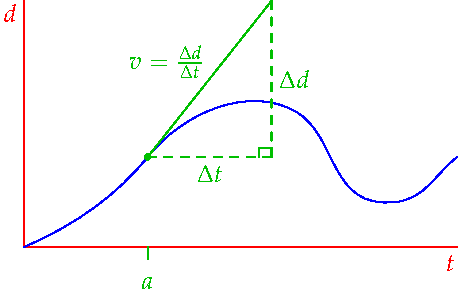
\includegraphics{diff-history}
		&
		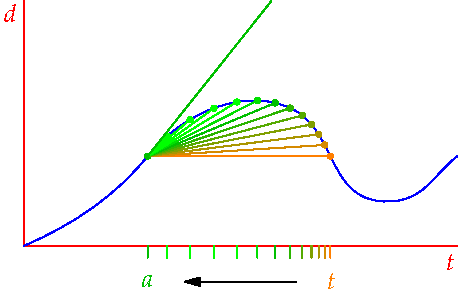
\includegraphics{diff-history2}
		\\
		\centering Instantaneous velocity equals constant velocity corresponding to tangent line
		&
		\centering Secant lines approximate tangent line as $t\to a$
	\end{tabular}
\end{center}

The average velocity of the particle over the time interval $[a,t]$ is the slope of the secant line, namely
\[
	v_\text{av}(a,t)=\frac{d(t)-d(a)}{t-a}
\]
Since the secant lines approximate the tangent line as $t$ approaches $a$, it seems  reasonable that we should compute the instantaneous velocity in this manner:
\[
	v(a)=\lim_{t\to a}v_\text{av}(a,t)
	=\lim_{t\to a}\frac{d(t)-d(a)}{t-a}
\]
This is, of course, the modern definition of the \emph{derivative.}
\goodbreak


\setcounter{subsection}{27}
\subsection{Basic Properties of the Derivative}\label{sec:derivproperties}

\begin{defn}{}{deriv}
	Let $f:U\to\R$ and $a\in U^\circ$ an \textbf{interior point}. We say that \emph{$f$ is differentiable at $a$} if the following limit exists (is \emph{finite}!)
	\[
		\lim_{x\to a}\frac{f(x)-f(a)}{x-a}
	\]
	We call this limit the \emph{derivative of $f$ at $a$} and denote its value by $\diffat[f]{x}{x=a}$ or $f'(a)$.\smallbreak
	If $f'(a)$ exists for all $a\in U$ then $f$ is \emph{differentiable (on $U$)}; the derivative becomes a function $\textcolor{Green}{f'(x)}=\textcolor{red}{\diff[f]{x}}$.
\end{defn}

The two notations are partly attributable to the primary founders of calculus: \textcolor{Green}{Issac Newton} and \textcolor{red}{Gottfried Leibniz}. Each has its pros and cons and you should be comfortable with both.

\boldinline{One-sided derivatives} 

Differentiability only makes sense at interior points of $U$ since the defining limit is two-sided. \emph{Left-} and \emph{right-derivatives} may be defined using one-sided limits; differentiability is then equivalent to these being equal. All results in this section hold for one-sided derivatives with suitable (sometimes tedious) modifications. It is common, though strictly incorrect, to say that $f$ is differentiable on $[a,b)$ if it is differentiable on the interior $(a,b)$ and \emph{right-}differentiable at $a$. In these notes we will strictly adhere to Definition \ref{defn:deriv}: differentiable means \emph{two-sided.}


\begin{examples}{}{}
	Basic examples should be familiar from elementary calculus.
	\begin{enumerate}
	  \item Let $f(x)=x^2+4x$. Then, for any $a\in\R$,
		\begin{align*}
			\lim_{x\to a}\frac{f(x)-f(a)}{x-a}
			&=\lim_{x\to a}\frac{x^2+4x-a^2-4a}{x-a} 
			=\lim_{x\to a}\frac{(x-a)(x+a+4)}{x-a}\\
			&=\lim_{x\to a}(x+a+4)=2a+4
		\end{align*}
		Note how the definition of $\lim\limits_{x\to a}$ allows us to cancel the $x-a$ terms from the numerator and denominator. We conclude that $f$ is differentiable (on $\R$) and that $f'(x)=2x+4$.
		
		\item Let $g(x)=\frac{x+1}{2x-3}$. Then, for any $a\neq\frac 32$,
		\begin{align*}
			\lim_{x\to a}\frac{f(x)-f(a)}{x-a}
			&=\lim_{x\to a}\frac 1{x-a}\left[\frac{x+1}{2x-3}-\frac{a+1}{2a-3}\right] 
			=\lim_{x\to a}\frac{5a-5x}{(x-a)(2x-3)(2a-3)}\\
			&=\lim_{x\to a}\frac{-5}{(2x-3)(2a-3)} 
			=\frac{-5}{(2a-3)^2}
		\end{align*}
		$f$ is therefore differentiable on its domain $\R\setminus\{\frac 32\}$ with derivative $f'(x)=\frac{-5}{(2x-3)^2}$.
	\end{enumerate}
\end{examples}

The familiar expressions
\[
	f'(a)=\lim_{h\to 0}\frac{f(a+h)-f(a)}h,\qquad 
	f'(x)=\lim_{h\to 0}\frac{f(x+h)-f(x)}h
\]
are equivalent to the original definition (Exercise \ref{ex:hderiv}). While seemingly simpler, they sometimes lead to nastier calculations: see what happens if you try the previous example in this language\ldots\medbreak\goodbreak

We now turn to perhaps the most well-known result of elementary calculus.

\begin{thm}{Power Law}{}
	Let $r\in\R$. Then $f(x)=x^r$ is differentiable with $f'(x)=rx^{r-1}$.
\end{thm}

The domains of $f$ and $f'$ depend messily on $r$, but the formula holds at least on the interval $(0,\infty)$. We leave a complete proof to the exercises and instead consider a few generalizable examples.

\begin{examples}{}{}
	\exstart If $n\in\N$ and $a\in\R$, a simple factorization yields
	\begin{align*}
		\lim_{x\to a}\frac{x^n-a^n}{x-a}
		&=\lim_{x\to a}\frac{(x-a)(x^{n-1}+ax^{n-2}+\cdots +a^{n-2}x+a^{n-1})}{x-a}\tag{$\ast$}\\
		&=\lim_{x\to a}(x^{n-1}+ax^{n-2}+\cdots +a^{n-2}x+a^{n-1}) 
		=na^{n-1}
	\end{align*}
	We conclude that $\diff x x^n=nx^{n-1}$.
	\begin{enumerate}\setcounter{enumi}{1}
		\begin{minipage}[t]{0.68\linewidth}\vspace{0pt}
			\item If \textcolor{blue}{$f(x)=x^{-1}$} and $a\neq 0$, then
			\begin{align*}
				\lim_{x\to a}\frac{x^{-1}-a^{-1}}{x-a}
				&=\lim_{x\to a}\frac{a-x}{ax(x-a)} 
				=\lim_{x\to a}\frac{-1}{ax}=-\frac 1{a^2}
			\end{align*}
			from which we conclude that \textcolor{Green}{$f'(x)=-x^{-2}$}.\smallbreak
			A similar approach followed by the factorization ($\ast$) proves the power law for all negative integer exponents:
			\[
				\frac{x^{-n}-a^{-n}}{x-a}=\frac{a^n-x^n}{a^nx^n(x-a)}=\cdots
			\]
		\end{minipage}
		\hfill
		\begin{minipage}[t]{0.3\linewidth}\vspace{-10pt}
			\flushright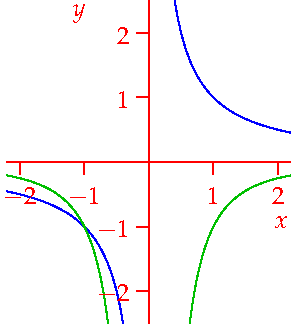
\includegraphics[scale=0.95]{diff-exneg2}
		\end{minipage}
		\bigbreak
	
		\begin{minipage}[t]{0.7\linewidth}\vspace{0pt}
			\item To differentiate $x^{1/n}$, substitute $x=y^n$ and observe case 1. For instance, if \textcolor{purple}{$g(x)=x^{1/3}$} and $a\neq 0$, then $y=x^{1/3}$ and $b=a^{1/3}$ yield
			\begin{align*}
				\lim_{x\to a}\frac{x^{1/3}-a^{1/3}}{x-a}&= \lim_{y\to b}\frac{y-b}{y^3-b^3} = \frac 1{3b^2}=\frac 13a^{-2/3}\\
				&\implies \textcolor{orange}{g'(x)=\frac 13x^{-2/3}}
			\end{align*}
			Note that $g$ is \emph{not} differentiable at $x=0$!
		\end{minipage}\begin{minipage}[t]{0.3\linewidth}\vspace{0pt}
			\flushright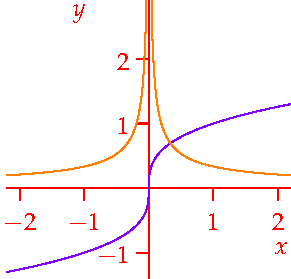
\includegraphics[scale=0.95]{diff-exthird}
		\end{minipage}
	\end{enumerate}
	\hangindent0pt We could similarly compute the derivative for all rational exponents, though it is much easier to wait for the chain rule. The power law for irrational exponents is somewhat more ticklish.
\end{examples}


\begin{cor}{Basic Transcendental Functions}{}
	Recalling our development of power series in Chapter \ref{chap:series}, the power law (for positive integers!) is all we need to see that
	\[
		\diff x\exp(x)=\exp(x),\qquad 
		\diff x\sin x=\cos x,\qquad 
		\diff x\cos x=-\sin x
	\]
\end{cor}

It is also possible to develop these results independently of power series (see e.g.\ Exercise \ref{ex:trigdiff}).
\goodbreak


\boldsubsubsection{Failure of differentiability} 

It is instructive to consider how a function might fail to be differentiable. Firstly, a familiar fact shows that functions are not differentiable at discontinuities.

\begin{lemm}{}{}
	If $f$ is differentiable at $a$ then $f$ is continuous at $a$.
\end{lemm}

\begin{proof}
	Just take the limit (think carefully why this works!):
	\[
		\lim_{x\to a}f(x)
		=\lim_{x\to a}\left[\frac{f(x)-f(a)}{x-a}(x-a)+f(a)\right] 
		=f'(a)(0-0)+f(a) 
		=f(a)\tag*{\qedhere}
	\]
	%The first term approaches $f'(a)\cdot\lim\limits_{x\to a}(x-a)=0$ since $f'(a)$ is defined and finite.
\end{proof}

It remains to consider situations when a function is continuous but not differentiable.

\begin{examples}{}{nondiff}
	The following exemplify all situations where a function is continuous on an interval and differentiable everywhere except at a single interior point. As with isolated discontinuities, these are classified by considering the three ways in which the derivative limit might not converge. 
	\begin{enumerate}
		\item A \emph{vertical tangent line} occurs when the limit is infinite. For instance, $g(x)=x^{1/3}$ at $x=0$. 
		
	  \item\label{ex:nondiff2} \emph{Corners} occur when the one-sided limits are unequal (could be infinite). For instance, $f(x)=\nm x$ is not differentiable at zero, with one-sided limits
	  \begin{gather*}
		  \lim_{x\to 0^+}\frac{\nm x-\nm 0}{x-0}=\lim_{x\to 0^+}\frac xx =1\neq
		  \lim_{x\to 0^-}\frac{\nm x-\nm 0}{x-0}=\lim_{x\to 0^-}\frac{-x}x =-1
	  \end{gather*}
		Indeed $f$ is differentiable everywhere except at zero, with
	  \[
	  	f'(x)=
	  	\begin{cases}
				1&\text{if }x>0\\
				-1&\text{if }x<0
			\end{cases}
		\]
		A \emph{cusp} describes the special case where the one-sided limits are $\infty\neq-\infty$. 
	
		\begin{minipage}[t]{0.64\linewidth}\vspace{0pt}
		  \item\label{ex:nondiff3} A \emph{singularity} is where left- and/or right-limits do not exist. The standard example is
		  \[
		  	f(x)=
		  	\begin{cases}
		  		x\sin\frac 1x&\text{if }x\neq 0\\
		  		0&\text{if }x=0
		  	\end{cases}
		  \]
		  which is continuous on $\R$ and differentiable everywhere except at zero: the details are in Exercise \ref{ex:diffnonzero}.
	  \end{minipage}
	  \hfill
	  \begin{minipage}[t]{0.34\linewidth}\vspace{0pt}
	  	\flushright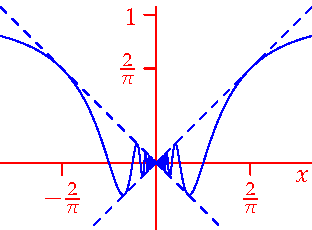
\includegraphics[scale=0.95]{unifcontex2}
	  \end{minipage}
	\end{enumerate}
	\hangindent0pt Singularities and vertical tangent lines can also prevent one-sided differentiability.
\end{examples}

More esoteric examples of non-differentiability are possible:
\begin{itemize}
  \item Utilizing series, we can create functions which are continuous on an interval but \emph{nowhere differentiable}! For an example, see Exercise \ref{exs:strangefunction}.
  \item It is also possible to construct a function which differentiable (and thus continuous) at precisely one point; can you think of an example?
\end{itemize}

\goodbreak


\boldsubsubsection{The Basic Rules of Differentiation}
	
\begin{thm}{}{basicdiff}
	Let $f,g$ be differentiable and $k,l$ be constants.
	\begin{enumerate}
	  \item (Linearity)\quad The function $kf+lg$ is differentiable with $(kf+lg)'=kf'+lg'$.
	  \item (Product rule)\quad The function $fg$ is differentiable with $(fg)'=f'g+fg'$.
	  \item (Inverse functions)\quad If $f$ is bijective with non-zero derivative, then $f^{-1}$ is differentiable and
		\[
			\diff yf^{-1}(y)=\frac 1{f'\big(f^{-1}(y))\big)}
		\] 
	\end{enumerate}
\end{thm}

\begin{proof}
Parts 1 and 2 follow from the limit laws:
\begin{gather*}
	\lim_{x\to a}\frac{(kf+lg)(x)-(kf+lg)(a)}{x-a}=\lim_{x\to a}\left[k\frac{f(x)-f(a)}{x-a}+l\frac{g(x)-g(a)}{x-a}\right]=kf'(a)+lg'(a)\\
	\lim_{x\to a}\frac{f(x)g(x)-f(a)g(a)}{x-a}=\lim_{x\to a}\left[\frac{f(x)-f(a)}{x-a}g(x)+f(a)\frac{g(x)-g(a)}{x-a}\right]=f'(a)g(a)+f(a)g'(a)
\end{gather*}
Note where we used the continuity of $g$ in the second line ($\lim g(x)=g(a)$). Part 3 is an exercise.
\end{proof}

The inverse function rule should be intuitive: since the graphs of $f$ and $f^{-1}$ are related by reflection in the diagonal $y=x$, gradients at corresponding points are reciprocals. The result feels even more natural in Leibniz's notation: $\diff[x]{y}=\frac 1{\dy/\dx}$.

\begin{examples}{}{}
	\exstart Linearity permits the differentiation of any polynomial: e.g.,
	\[
		\diff x\big(7x^2+13x^4\big)=7\diff xx^2+13\diff xx^4=14x+52x^3
	\]
	\begin{enumerate}\setcounter{enumi}{1}
		\item The product rule extends the reach of differentiation to include simple combinations: e.g.,
		\[
			\diff x(x^4\sin x) =\left(\diff xx^4\right)\sin x+x^4\diff x\sin x = 4x^3\sin x-x^4\cos x
		\]
		
		\item Inverse trigonometric functions can now be differentiated: e.g.,
		\[
			y=\sin^{-1}x\implies 
			\diff x\sin^{-1}x=\diff[y]{x}
			=\left(\diff[x]{y}\right)^{-1}
			=\frac 1{\cos y}
			=\frac 1{\sqrt{1-\sin^2\!y}}
			=\frac 1{\sqrt{1-x^2}}
		\]
		
		\item Define the natural logarithm to be the inverse of the (bijective!) exponential function $\exp(x)$:
		\[
			y=\ln x\iff x=\exp y
		\]
		It follows that
		\[
			\diff x\ln x=\left(\diff[x]{y}\right)^{-1}
			=\frac 1{\exp y}=\frac 1x
		\]
		The full details, and the justification that $\exp x=e^x$, are in Exercise \ref{exs:expmasochist}.
	\end{enumerate}
\end{examples}
\goodbreak


\begin{thm}{Chain Rule}{}
	If $g$ is differentiable at $a$, and $f$ is differentiable at $g(a)$, then $f\circ g$ is differentiable at $a$ with derivative
	\[
		(f\circ g)'(a)=f'\big(g(a)\big)\,g'(a)
	\]
\end{thm}

In Leibniz's notation, $\diff[(f\circ g)]{x}=\diff[f]{g}\diff[g]{x}$: this \emph{looks} like a simple cancellation of the $\dg$ terms\ldots\footnote{%
	This is completely unjustified since $\dg$ does not (for us) have independent meaning. The same problem appears in a famously flawed one-line `proof' of the chain rule:
	\[
		\lim_{x\to a}\frac{f\big(g(x)\big)-f\big(g(a)\big)}{x-a} 
		\overset{\text{?}}{=} \lim_{x\to a}\textcolor{blue}{\frac{f\big(g(x)\big)-f\big(g(a)\big)}{g(x)-g(a)}} \lim_{x\to a}\frac{g(x)-g(a)}{x-a}
	\]
	The \textcolor{blue}{second limit} doesn't make sense unless $g(x)\neq g(a)$ for all $x$ on some punctured neighborhood of $a$: in particular, $g(x)$ cannot be \emph{constant}! The faulty argument may be repaired by replacing this \textcolor{blue}{difference quotient} with $f'\bigl(g(a)\bigr)$ whenever $g(x)=g(a)$, \emph{before} taking the limit. This is precisely what $\gamma\bigl(g(x)\bigr)$ does in the correct proof.%
}



\begin{proof}
	Since $f$ and $g$ are differentiable, $a$ is interior to $\dom(g)$ and $g(a)$ is interior to $\dom(f)$. Since $g$ is continuous at $a$, there must exist some open interval $U\ni a$ for which $x\in U\Longrightarrow g(x)\in\dom(f)$.\par
	Define $\gamma:\dom(f)\to\R$ via
	\[
		\gamma(v)=
		\begin{cases}
			\frac{f\big(v\big)-f\big(g(a)\big)}{v-g(a)}&\text{if }v\neq g(a)\\
			f'\big(g(a)\big)&\text{if }v=g(a)
		\end{cases} 
		\tag{$\ast$}
	\]
	Since $f$ is differentiable at $g(a)$,we see that $\gamma$ is continuous there: indeed $\smash[b]{\lim\limits_{v\to g(a)}\gamma(v)=f'\bigl(g(a)\bigr)}$.\par
	For any $x\in U\setminus\{a\}$, let $v=g(x)$ in ($\ast$). Then
	\[
		\frac{f\big(g(x)\big)-f\big(g(a)\big)}{x-a}
		=\gamma\bigl(g(x)\bigr)\frac{g(x)-g(a)}{x-a}
	\]
	Take limits as $x\to a$ for the result.
\end{proof}

\begin{cor}{Quotient Rule}{quotinv1}
	Suppose $f$ and $g$ are differentiable. Then $\frac fg$ is differentiable whenever $g(x)\neq 0$. Moreover
	\[
		\left(\frac fg\right)'=\frac{f' g-fg'}{g^2}
	\]
\end{cor}

The proof is an exercise.

\begin{examples}{}{}
	\exstart By the quotient rule,
		\[
			\diff x\tan x=\diff x\frac{\sin x}{\cos x}
			=\frac{\cos^2\!x+\sin^2\!x}{\cos^2\!x}=\sec^2\!x
		\]
	\begin{enumerate}\setcounter{enumi}{1}
		\item We can now differentiate highly involved combinations of elementary functions:
		\[
			\diff x\left[\tan(e^{4x^2})-\frac{7x}{\sin x}\right]
			=8xe^{4x^2}\sec^2(e^{4x^2})-\frac{7\sin x-7x\cos x}{\sin^2\!x}
		\]
	\end{enumerate}
\end{examples}

\goodbreak


\begin{exercises}{}
	\exstart Use Definition \ref{defn:deriv} to calculate the derivatives.
	\begin{enumerate}\setcounter{enumi}{1}
		\item[]\begin{enumeratea}
		  \item \makebox[180pt][l]{$f(x)=x^3$ \ at $x=2$ \hfill(b)}
			\space $g(x)=x+2$ \ at $x=a$
			\item[(c)] \makebox[180pt][l]{$f(x)=x^2\cos x$ \ at $x=0$ \hfill(d)}
			\space $r(x)=\frac{3x+4}{2x-1}$ \ at $x=1$
		\end{enumeratea}
	  
	  
	  \item Differentiate the function $f(x)=\cos\bigl(e^{x^5-3x}\bigr)$ using the chain and product rules.
	  
	  
	  \item\begin{enumerate}
	    \item Prove the quotient rule (Corollary \ref{cor:quotinv1}) by combining the chain and product rules.
	  	\item Prove the inverse derivative rule (Theorem \ref{thm:basicdiff}, part 3).\par
	  	(\emph{Hint: You can't simply differentiate $1=\diff[x]x=\diff xf\bigl(f^{-1}(x)\bigr)$ using the chain rule; why not?})
	  \end{enumerate}
	  
	  
	  \item\begin{enumerate}
	    \item Find the derivatives of secant, cosecant and cotangent using the quotient rule.
	    \item Why did we choose the positive square-root when computing $\diff x\sin^{-1}x$? What is the standard domain of arcsine, and what happens at $x=\pm 1$?
	    \item Find the derivatives of the inverse trigonometric functions using the inverse function rule.
	  \end{enumerate}
	  
	  
	  \item\label{ex:hderiv} Using the definition of the derivative, and supposing that $f$ is differentiable at $a$, prove that
	  \[
	  	f'(a)=\lim_{h\to 0}\frac{f(a+h)-f(a)}{h}=\lim_{h\to 0}\frac{f(a+h)-f(a-h)}{2h}
	  \]
	  
	  
   	\item Use induction to prove the power law $\diff xx^n=nx^{n-1}$ when $n\in\N$ using \emph{only} the product rule and the fact that $\diff xx=1$.
   		  
	  
	  \item Prove that $f(x)=x\nm x$ is differentiable everywhere and compute its derivative.
	  
	  
	  \item Show that $f(x)=x^{2/3}$ has a \emph{cusp} (see Example \ref*{ex:nondiff}.\ref{ex:nondiff2}) at $x=0$.
	  	  
	  
	  \item\label{exs:diffdiscont} Show that following function is differentiable everywhere and compute its derivative:
	  \[
	  	f(x)=
	  	\begin{cases}
	  		x^2\sin\frac 1x&\text{if }x\neq 0\\
	  		0&\text{if }x=0
	  	\end{cases}
	  \]
	  Moreover, prove that the derivative $f'$ is \emph{discontinuous} at $x=0$.
	  
	  
	  \item\label{ex:diffnonzero} Prove that the function in Example \ref*{ex:nondiff}.\ref{ex:nondiff3}
	  is differentiable everywhere \emph{except} at $x=0$.
	  
	  
	  \item Suppose $f(x)=x^2$ whenever $x\in\Q$ and $f(x)=0$ whenever $x\not\in\Q$. At what values of $x$ is $f$ differentiable? Prove your assertion.
	  
	
		\begin{minipage}[t]{0.63\linewidth}\vspace{0pt}
		  \item\label{ex:trigdiff}\begin{enumerate}
		    \item Suppose $0<h<\frac\pi 2$. Use the picture to show that
				\[
					0<\frac{1-\cos h}h< \sin\frac{h}2 
					\quad\text{and}\quad  
					\sin h< h<\tan h
				\]
				Hence conclude that $\lim\limits_{h\to 0}\frac{\sin h}h=1$ and $\lim\limits_{h\to 0}\frac{1-\cos h}h=0$.
			\item Use part (a) to prove that $\diff x\sin x=\cos x$
		\end{enumerate}
		\end{minipage}
		\hfill
		\begin{minipage}[t]{0.36\linewidth}\vspace{0pt}
	  	\flushright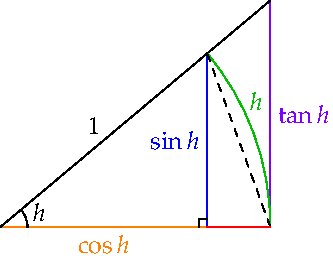
\includegraphics[scale=0.95]{trig-diff2}
	  \end{minipage}
	  
	
   	\item (Hard)\lstsp Use induction to prove the Leibniz rule (general product rule):
   	\[
   		(fg)^{(n)}=\sum_{k=0}^n\binom nk f^{(k)}g^{(n-k)}
   	\]
   
   	\goodbreak
   	
   	\item[]\textbf{Warning!} The last two exercises are much longer and \& tougher: have a go if you appreciate a challenge.
   	
   	\item\label{exs:expmasochist} \textbf{The Exponential Function \& the Power Law}\smallbreak
    	The ratio tests shows that the power series $\exp(x):=\sum_{n=0}^\infty\frac{x^n}{n!}$ converges for all real $x$. 
%Via term-by-term differentiation, this function moreover satisfies the initial value problem
%   	\[
%   		\diff x\exp(x)=\exp(x),\qquad \exp(0)=1
%   	\]
		\emph{Define} $e:=\exp(1)$. Certainly $e^x$ makes sense whenever $x\in\Q$. If $x$ is irrational, instead define
	  \[
	  	e^x:=\sup\{e^q:q\in\Q,\ q< x\}
	  \]
		The goal of this question is to \emph{prove} that $\exp(x)=e^x$. As a nice bonus we recover Bernoulli's limit identity $e=\lim\limits_{n\to\infty}\left(1+\frac 1n\right)^n$ and obtain a complete proof of the power law!
	  \begin{enumerate}
	    \item For all $x,y\in\R$, prove that $\exp(x+y)=\exp(x)\exp(y)$\par
	    (\emph{Hint: use the binomial theorem and change the order of summation})
	    
	    \item Show that $\exp(x)$ is always positive, \emph{even when $x<0$.}
	    
	    \item Prove that $\exp:\R\to (0,\infty)$ is bijective.\par
	    (\emph{Hint: $x\ge 0\Longrightarrow \exp(x)\ge 1+x$; take limits then apply part (a)})
	    
	    \item Prove that $e^x=\exp(x)$. Do this in three stages:
	    \begin{itemize}
	      \item If $x\in\N$, use part (a). Now check for $x\in\Z^-$.
	      \item If $x=\frac mn\in\Q$, first compute $\left[\exp(\frac mn)\right]^n$.
	      \item If $x$ is irrational, consider a sequence of rational numbers $q_n<x$ with $e^{q_n}\to e^x$\ldots
	    \end{itemize}
	
	    \item Let $\ln:(0,\infty)\to\R$ be the inverse function of $\exp$. Prove the logarithm laws:
	    \[
	    	\ln(xy)=\ln x+\ln y
	    	\quad\text{and}\quad 
	    	\ln x^r=r\ln x
	    \]
	    (\emph{Just do this when $r\in\N$; in general, another argument like part (d) is required})
	    
	    \item We've already seen that $\diff y\ln y=\frac 1y$. Use the fact that
	    \[
	    	\diff y\ln y=\lim_{h\to 0}\frac{\ln(y+h)-\ln y}h
	    \]
	    to prove that $\exp(x)=\lim\limits_{n\to\infty}\left(1+\frac xn\right)^n$, thus recovering Bernoulli's definition of $e$.
	    
			\item For any $r\in\R$, \emph{define} $x^r:=\exp(r\ln x)$. Hence obtain the power law for any exponent.
   	\end{enumerate}
   	
   	
   	\goodbreak
   	
   	
  	\item\label{exs:strangefunction} \textbf{A Very Strange Function}\smallbreak
  	Here is a classic example of a continuous but nowhere-differentiable function!\smallbreak

		Let $f$ be the \emph{sawtooth} function defined by \textcolor{Green}{$f(x)=\nm x$} whenever $x\in[-1,1]$ and extending periodically to $\R$ so that \textcolor{Green}{$f(x+2)=f(x)$}. Now define $\textcolor{blue}{g}:\R\to\R$ via
  	\[
  		\textcolor{blue}{g(x)=\sum_{n=0}^\infty \left(\frac 34\right)^nf(4^nx)}
  	\]
  	\vspace{-30pt}
	  \begin{center}
		  \begin{tabular}{c@{\qquad}c}
			  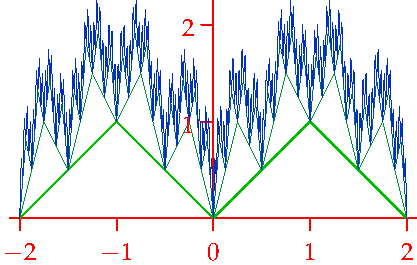
\includegraphics[scale=0.95]{sawtooth}
			  &
			  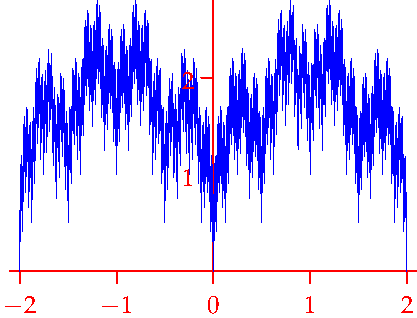
\includegraphics[scale=0.95]{sawtooth2}\\
			  $f(x)$ and iterations to $n=3$
			  &
			  $g(x)$ (really $n=6$, but can you tell?!)
		  \end{tabular}
	  \end{center}
  
  \begin{enumeratea}
    \item Prove that $g$ is well-defined and continuous on $\R$.
    \item Let $x\in\R$ and $m\in\N$ be fixed. Define $h_m=\pm\frac 12\cdot 4^{-m}$ where the sign is chosen so that no integers lie strictly between $4^mx$ and $4^m(x+h_m)=4^mx\pm\frac 12$.\smallbreak
    For each $n\in\N_0$, define
    \[
    	k_n =\frac{f\big(4^n(x+h_m)\big)-f(4^nx)}{h_m}
    \]
    Prove the following
    \begin{enumerate}
      \item[i.] $\nm{k_n}\le 4^n$ with equality when $n=m$.
      \item[ii.] $n>m\Longrightarrow k_n=0$.
    \end{enumerate}
    (\emph{Hint: $\nm{f(y)-f(z)}\le\nm{y-z}$: when is this an equality?})

    \item Use part (b) to prove that
    \[
    	\nm{\frac{g(x+h_m)-g(x)}{h_m}}\ge \frac 12(3^m+1)
    \]
    Hence conclude that $g$ is \emph{nowhere differentiable.}
  \end{enumeratea}
   
	\end{enumerate}
\end{exercises}



\clearpage



\subsection{The Mean Value Theorem}\label{sec:mvt}

A key result in elementary calculus, this should be very familiar from your previous studies.

\begin{thm}{Mean Value Theorem/MVT}{}
	Let $f$ be continuous on $[a,b]$ and differentiable on $(a,b)$. Then there exists $\xi\in(a,b)$ such that $f'(\xi)=\frac{f(b)-f(a)}{b-a}$.
\end{thm}

This follows easily from two lemmas.

\begin{lemm}{}{rolle}
	\exstart (Critical Points)\quad Suppose $g$ is bounded on $(a,b)$ and attains its maximum or minimum at $\xi\in(a,b)$. If $g$ is differentiable at $\xi$ then $g'(\xi)=0$. \vspace{-5pt} %If $g$ is differentiable at $\xi$ then $g'(\xi)=0$.
	\begin{enumerate}\setcounter{enumi}{1}%\itemsep0pt
	  \item (Rolle's Theorem)\quad Suppose $g$ is continuous on $[a,b]$, differentiable on $(a,b)$, and $g(a)=g(b)$. Then there exists $\xi\in(a,b)$ such that $g'(\xi)=0$. 
	\end{enumerate}
\end{lemm}

The main result is obtained by applying Rolle's theorem to
\[
	g(x)=f(x)-\frac{f(b)-f(a)}{b-a}(x-b)
\]
and observing that $g(a)=f(b)=g(b)$ and $g'(x)=f'(x)-\frac{f(b)-f(a)}{b-a}$.

\begin{center}
	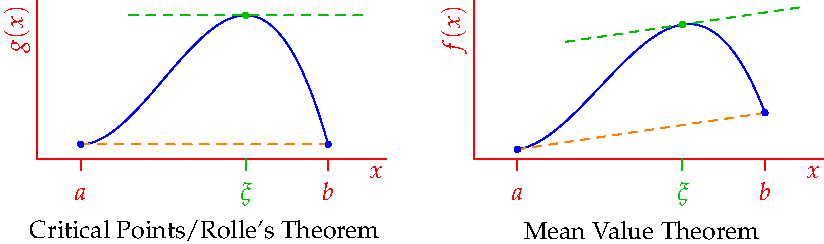
\includegraphics[scale=0.95]{mvt}
\end{center}

In the pictures, the orange and green lines are \emph{parallel}: the \textcolor{orange}{average slope} over the interval $[a,b]$ equals the \textcolor{Green}{gradient/derivative} $f'(\xi)$.

\begin{proof}[Proof of Lemma]
	\begin{enumerate}\itemsep0pt
	  \item For contradiction, suppose that
		\[
			g'(\xi)=\lim_{x\to \xi}\frac{g(x)-g(\xi)}{x-\xi}>0
		\]
		Let $\epsilon=g'(\xi)$ in the definition of limit: $\exists\delta>0$ such that
		\[
			0<\nm{x-\xi}<\delta
			\implies\nm{\frac{g(x)-g(\xi)}{x-\xi}-g'(\xi)}<g'(\xi)
			\implies 0<\frac{g(x)-g(\xi)}{x-\xi}<2g'(\xi)
		\]
		In particular, if $x\in(\xi,\xi+\delta)$, then $g(x)>g(\xi)$, contradicting maximality at $\xi$.\smallbreak
		The argument when $g'(\xi)<0$ is similar. Finally, apply to $-g$ for the result at a minimum.
	  \item By the Extreme Value Theorem (\ref{thm:cont2}), $g$ is bounded and attains its bounds.
	  If the extrema \emph{both} occur at the endpoints $a,b$, then $g$ is constant: any $\xi\in(a,b)$ satisfies the result.	Otherwise, at least one extreme occurs at some $\xi\in(a,b)$: part 1 says that $g'(\xi)=0$.\hfill\qedhere
	\end{enumerate}
\end{proof}
\goodbreak


\begin{examples}{}{}
	\exstart Let $f(x)=(x-1)^2(4-x)+x$ on $[a,b]=[1,4]$: this is roughly the above picture illustrating the mean value theorem. Compute the average slope and the derivative,
	\[
		\frac{f(b)-f(a)}{b-a}=1,\qquad 
		f'(x)=2(x-1)(4-x)-(x-1)^2+1 =-3x^2+12x-8
	\]
	and observe that
	\[
		f'(\xi)=\frac{f(b)-f(a)}{b-a}\iff 3\xi^2-12\xi+9=0\iff \xi=1\text{ or }3
	\]
	Since only 3 lies in the interval $(1,4)$, this is the value $\xi$ satisfying the mean value theorem.
	\begin{enumerate}\setcounter{enumi}{1}
	  \item We find the maximum and minimum values of $g(x)=x^4-14x^2+24x$ on the interval $[0,2]$.\vspace{-8pt}
	  
	  \begin{minipage}[t]{0.68\linewidth}\vspace{0pt}
	  The function is differentiable, with
	  \[
	  	g'(x)=4x^3-28x+24=4(x-2)(x-1)(x+3)
	  \]
	  By the Lemma, the locations of the extrema are either the endpoints $x=0,2$ or locations with zero derivative ($x=1$). Since
	  \[
	  	f(0)=0,\quad f(1)=11,\quad f(2)=8
	  \]
	  we conclude that $\max(f)=f(1)=11$ and $\min(f)=f(0)=0$.
	  \end{minipage}
	  \hfill
	  \begin{minipage}[t]{0.31\linewidth}\vspace{0pt}
	  	\flushright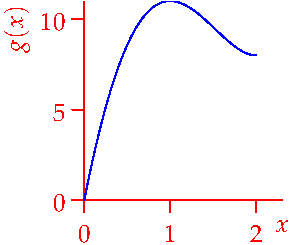
\includegraphics[scale=0.95]{mvt-ex}
	  \end{minipage}
	%   
	% 	\item Many values of $\xi$ can satisfy the Mean Value or Rolle's Theorem. For instance, if $f(x)=\sin x$ on the interval $[0,10\pi]$, then
	% 	\[\frac{f(10\pi)-f(0)}{10\pi-0}=\cos \xi=f'(\xi) \iff \xi=\frac\pi 2,\frac{3\pi}2,\ldots,\frac{19\pi}2\]
	\end{enumerate}
\end{examples}


\boldinline{Consequences of the Mean Value Theorem} Several simple corollaries relate to monotonicity.

\begin{defn}{}{}
	Suppose $f:I\to\R$ is defined on an interval $I$. We say that $f$ is:\vspace{-3pt}
	\begin{quote}\itemsep0pt
	  \emph{Increasing (monotone-up) on $I$} if $x<y\Longrightarrow f(x)\le f(y)$\smallbreak
	  \emph{Decreasing (monotone-down) on $I$} if $x<y\Longrightarrow f(x)\ge f(y)$
	\end{quote}
	\vspace{-3pt}
	We say \emph{strictly} increasing/decreasing if the inequalities are strict.
\end{defn}

\begin{examples}[lower separated=false, sidebyside, sidebyside align=top seam, sidebyside gap=0pt, righthand width=0.4\linewidth]{}{}
	\exstart $f:x\mapsto x^2$ is strictly increasing on $[0,\infty)$ and strictly decreasing on $(-\infty,0]$.
	\begin{enumerate}\setcounter{enumi}{1}
		\item The floor function $f:x\mapsto \lfloor x\rfloor$ (the greatest integer less than or equal to $x$) is increasing, but not strictly, on $\R$.
	\end{enumerate}
	\tcblower
  \flushright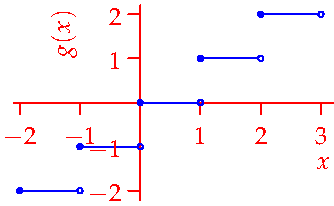
\includegraphics[scale=0.95]{mvt-floor}
\end{examples}

\begin{cor}{}{mvtincdec}
	Suppose $f$ is differentiable on an interval $I$. Then
	\begin{enumerate}
	  \item $f'\ge 0\text{ on }I\iff f\text{ is increasing on }I$
	  \item $f'\le 0\text{ on }I\iff f\text{ is decreasing on }I$
	  \item $f'=0\text{ on }I\iff f\text{ is constant on }I$
	\end{enumerate}
\end{cor}

\goodbreak

\begin{proof}
	\begin{description}
		\item[\normalfont (Part 1, $\Rightarrow$)] Let $x<y$ where $x,y\in I$. By the mean value theorem, $\exists\xi\in(x,y)$ such that
		\[
			\frac{f(y)-f(x)}{y-x}=f'(\xi)
			\quad\text{whence}\quad 
			f'(\xi)\ge 0\implies f(y)\ge f(x)
		\]
		\item[$(\Leftarrow)$] For the converse, use the definition of derivative: \smash{$f'(\xi)=\lim\limits_{x\to\xi}\frac{f(x)-f(\xi)}{x-\xi}$.} If $f$ is increasing, then
		\[
			x>\xi\implies f(x)\ge f(\xi)\implies f'(\xi)\ge 0
		\]
	\end{description}
	Parts 2 and 3 are similar.
\end{proof}

Corollary \ref{cor:mvtincdec} yields a couple of (hopefully familiar) flashbacks to elementary calculus.

\begin{cor}{}{1stderivtest}
	Let $I$ be an interval.
	\begin{enumerate}
	  \item (Anti-derivatives on an interval)\quad If $f'(x)=g'(x)$ on $I$, then $\exists c$ such that $g(x)=f(x)+c$ on $I$.
	  \item (First derivative test)\quad Suppose $f$ is continuous on $I$ and differentiable except perhaps at $\xi$. If
		\begin{gather*}
			\begin{cases}
			f'(x)<0&\text{whenever }x<\xi,\ \ \text{and}\\
			f'(x)>0&\text{whenever }x>\xi
			\end{cases}\quad \text{ then $f$ has its minimum value at $x=\xi$}
		\end{gather*}
		The statement for a maximum is similar.
	\end{enumerate}
\end{cor}


\begin{examples}{}{}
	\exstart Since $\diff x\sin(3x^2+x)=(6x+1)\cos(3x^2+x)$ on (the interval) $\R$, whence all anti-derivatives of $f(x)=(6x+1)\cos(3x^2+x)$ are given by
	\[
		\int f(x)\,\dx=\int (6x+1)\cos(3x^2+x)\,\dx=\sin(3x^2+x)+c
	\]
	As is typical in calculus, we use the \emph{indefinite integral} notation $\int f(x)\,\dx$ for anti-derivatives.
	\begin{enumerate}\setcounter{enumi}{1}
	  \begin{minipage}[t]{0.6\linewidth}\vspace{0pt}
	  	\item If $f(x)=x^{2/3}e^{x/3}$, then $f'(x)=\frac 13x^{-1/3}(2+x)e^{x/3}$.\smallbreak
	  	By Lemma \ref{lemm:rolle}, the only possible critical points are at $x=0$ or $-2$. The sign of the derivative is also clear:
	  	\begin{center}
	  		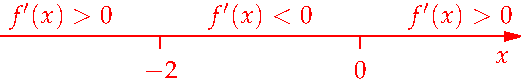
\includegraphics[scale=0.95]{mvt-ex3}
	  	\end{center}
	  \end{minipage}
	  \hfill
	  \begin{minipage}[t]{0.39\linewidth}\vspace{0pt}
	  	\flushright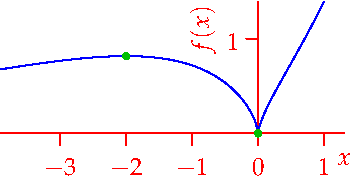
\includegraphics[scale=0.95]{mvt-ex2}
	  \end{minipage}
	  \smallbreak	
		By the 1\st{} derivative test, $f$ has a maximum at $x=-2$ and a minimum at $x=0$.
	\end{enumerate}
\end{examples}

We finish this section by tying together the mean and intermediate value theorems.

\begin{thm}{IVT for Derivatives}{intvalderiv}
	Suppose $f$ is differentiable on an interval $I$ containing $a<b$, and that $L$ lies between $f'(a)$ and $f'(b)$. Then $\exists\xi\in(a,b)$ such that $f'(\xi)=L$.
\end{thm}

If $f'(x)$ is \emph{continuous,} this is just the intermediate value theorem applied to $f'$; surprisingly, continuity of $f'$ is \emph{not} required. A full proof is in Exercise \ref{exs:ivtderivs}.

\goodbreak


% \begin{proof}
% Define $g:I\to\R$ by $g(x)=f(x)-Lx$ and let $\xi\in[a,b]$ be such that\footnote{$g$ differentiable $\implies g$ continuous on the bounded interval $[a,b]$. The extreme value theorem says $g$ is bounded and attains its bounds.}
% \[g(\xi)=\min\{g(x):x\in[a,b]\}\]
% If $\xi\in(a,b)$, Lemma \ref{lemm:rolle} says that $g'(\xi)=0\implies f'(\xi)=L$.\\[5pt]
% To complete the proof, we need to prove that $\xi\neq a$ or $b$. WLOG, assume that $f'(a)<f'(b)$. Then
% \[g'(a)=f'(a)-L<0<f'(b)-L=g'(b)\]
% In particular,
% \[\lim_{x\to a^+}\frac{g(x)-g(a)}{x-a}=g'(a)<0 \implies \exists \delta>0\text{ such that }a<x<a+\delta\implies g(x)<g(a)\]
% whence $g(a)$ is not the minimum value of $g$ on $[a,b]$. That $g(b)$ is not the minimum is similar.
% \end{proof}

% The classic example of a differentiable function with discontinuous derivative is
% \[f(x)=\begin{cases}
% x^2\sin(1/x)&x\neq 0\\
% 0&x=0
% \end{cases} \implies f'(x)=\begin{cases}
% 2x\sin(1/x)-\cos(1/x)&x\neq 0\\
% 0&x=0
% \end{cases}\]
% We leave the analysis of this to the homework.

% The derivative is discontinuous at $x=0$. We can still apply the theorem however. For instance, given $n\in\N$, let $a=0$ and $b=\frac 1{2\pi n}$ so that $f'(a)=0>f'(b)=-1$. If $L$ is any number in this interval, the theorem says
% \[\exists \xi_n\in\left(0,\frac 1{2\pi n}\right)\text{ such that }f'(x_n)=L\]
% With a little thinking, this says that the set of all possible limits $\lim\limits_{n\to\infty}f(x_n)$ taken over all sequences $x_n\to 0$ is in fact the interval $[-1,1]$!\goodbreak


% \begin{cor}{}{incdec}
% Suppose $f$ is differentiable on an interval and that $f'(x)\neq 0$. Then $f$ is either strictly increasing or strictly decreasing.
% \end{cor}
% 
% The proof is an easy exercise.

% \begin{proof}
% Suppose $a,b\in I$, that $f'(a)<0<f'(b)$. Then $\exists\xi$ such that $f'(\xi)=0$. Contradiction. it follows that 
% \end{proof}


\begin{exercises}
	\exstart Determine whether the conclusion of the mean value theorem holds for each function on the given interval. If so, find a suitable point $\xi$. If not, state which hypothesis fails.
	\begin{enumerate}\setcounter{enumi}{1}\itemsep0pt
	  \item[]\begin{enumerate}
	    \item \makebox[140pt][l]{$x^2$ on $[-1,2]$\hfill (b)}
	    \space\makebox[140pt][l]{$\sin x$ on $[0,\pi]$\hfill (c)}
	    \space $\nm x$ on $[-1,2]$
	    \item[(d)] \makebox[140pt][l]{$1/x$ on $[-1,1]$\hfill (e)}
	    \space $1/x$ on $[1,3]$
	  \end{enumerate}
	  
	  
	  \item Suppose $f$ and $g$ are differentiable on an interval $I$ containing $a<b$ and that $f(a)=f(b)=0$. By considering $h(x)=f(x)e^{g(x)}$, prove that $f'(\xi)+f(\xi)g'(\xi)=0$ for some $\xi\in (a,b)$.
	  
	  
	  \item Use the Mean Value Theorem to prove:\vspace{-5pt}
	  \begin{enumerate}
	    \item $x<\tan x$ for all $x\in(0,\frac\pi 2)$.
	    \item $\frac{x}{\sin x}$ is a strictly increasing function on $(0,\frac\pi 2)$.
	    \item $x\le\frac{\pi}2\sin x$ for all $x\in[0,\frac\pi 2]$.
	  \end{enumerate}
	  
	  
	  \item Suppose that $\nm{f(x)-f(y)}\le (x-y)^2$ for all $x,y\in\R$. Prove that $f$ is a constant function.  
	  
		\item\begin{enumerate}
		  \item Prove that $f'>0$ on an interval $I\Longrightarrow f$ is \emph{strictly} increasing on $I$.
		  \item Show that the converse of part (a) is \emph{false.}
	  	\item Carefully prove the first derivative test (Corollary \ref{cor:1stderivtest}).
		\end{enumerate}
	% 	but the converse does not. For example, $f:x\mapsto x^3$ is strictly increasing on $\R$ with derivative $f'(x)=3x^2\ge 0$: clearly $f'(0)=0$.
		
		
	  \item\label{exs:fincdec} If $f$ is differentiable on an interval $I$ such that $f'(x)\neq 0$ for all $x\in I$, use the intermediate value theorem for derivatives to prove that $f$ is either strictly increasing or strictly decreasing.
	  
	  
	  \item\label{exs:ivtderivs} (Intermediate value theorem for derivatives)\quad Let $f,a,b$ and $L$ be as in Theorem \ref{thm:intvalderiv}, define $g:I\to\R$ by $g(x)=f(x)-Lx$, and let $\xi\in[a,b]$ be such that
		\[
			g(\xi)=\min\bigl\{g(x):x\in[a,b]\bigr\}
		\]
		\begin{enumerate}
		  \item Why can we be sure that $\xi$ exists? If $\xi\in(a,b)$, explain why $f'(\xi)=L$.
			\item Assume WLOG that $f'(a)<f'(b)$. Prove that $g'(a)<0<g'(b)$. By considering $\lim\limits_{x\to a^+}\frac{g(x)-g(a)}{x-a}$, show that $\exists x>a$ for which $g(x)<g(a)$. Hence complete the proof.
		\end{enumerate}
	  
	  
	  \item Suppose $f'$ is differentiable on $(a,b)$, and is continuous except for a discontinuity at $c\in(a,b)$.
	  \begin{enumerate}
	    \item Obtain a contradiction if $\lim\limits_{x\to c^+}f'(x)=L<f'(c)$. Hence argue that $f'$ cannot have a \emph{removable} or a \emph{jump} discontinuity at $x=c$.\par
	    (\emph{Hint: let $\epsilon=\frac{f'(c)-L}2$ in the definition of limit and apply IVT for derivatives})
	    
	    \item Similarly, obtain a contradiction if \smash[b]{$\lim\limits_{x\to c^+}f'(x)=\infty$} and conclude that $f'$ cannot have an \emph{infinite} discontinuity at $x=c$.
	    
	  	\item It remains to see that $f'$ can have an essential discontinuity. Recall (Exercise \ref*{sec:derivproperties}.\ref{exs:diffdiscont}) that
			\[
				f:\R\to\R:x\mapsto 
				\begin{cases}
					x^2\sin\frac 1x&x\neq 0\\
					0&x=0
				\end{cases}
			\]
			is differentiable on $\R$, but has discontinuous derivative at $x=0$.
			\begin{enumerate}
	  		\item Use $x_n=\frac 1{2n\pi}$ and $y_n=\frac 1{(2n+1)\pi}$ to show that $f'$ has an essential discontinuity at $x=0$.
	  		\item Prove that if $\lim s_n=0$ and $\lim f'(s_n)=M$, then $M\in[-1,1]$.
				\item Prove that for any $L\in[-1,1]$, there is a sequence $(t_n)$ for which $\lim\limits f'(t_n)=L$.\par
				(\emph{Hint: Use IVT for derivatives\ldots})
			\end{enumerate}
	  \end{enumerate}
	\end{enumerate}
\end{exercises}


\goodbreak


\subsection{L'Hôpital's Rule}\label{sec:lhopital}

We are often required to consider \emph{indeterminate forms}: limits which do not yield easily to the standard limits laws. For instance, while it is tempting to write
\[
	\lim_{x\to 0}\frac{\sin 2x}{e^{3x}-1}
	=\frac{\lim\sin 2x}{\lim e^{3x}-1}
	=\frac 00 \tag{$\ast$}
\]
this is an incorrect application of the limit laws since the resulting quotient has no meaning.

\begin{defn}{}{indetform}
	An \emph{indeterminate form} is any limit where a naïve application of the limit laws results in a meaningless expression: the primary types are $\frac 00$, $\frac\infty\infty$, $\infty-\infty$, $0\cdot\infty$, $0^0$, $0^\infty$, and $1^\infty$.
\end{defn}

\begin{examples}{}{}
	\exstart $\lim\limits_{x\to 7^+}(x-7)^\frac 1{x-7}$ is an indeterminate form of type $0^\infty$.
	\begin{enumerate}\setcounter{enumi}{1}
	  \item Our motivating example $(\ast)$ may correctly be evaluated using the definition of the derivative:
		\[
			\lim_{x\to 0}\frac{\sin 2x}{e^{3x}-1}
			=\lim_{x\to 0}\frac{\sin 2x-0}{x-0}\frac{x-0}{e^{3x}-1} 
			=\left(\diffat x{x=0}\sin 2x\right) \left(\diffat x{x=0}e^{3x}\right)^{-1} 
			=\frac 23
		\]
		By considering $\lim\limits_{x\to 0}\frac{3a\sin 2x}{2(e^{3x}-1)}$, we see that an indeterminate form of type $\frac 00$ can take \emph{any value} $a$!
	\end{enumerate}
\end{examples}

The approach generalizes: if $f$ and $g$ are differentiable and $f(a)=0=g(a)$, then
\[
	\tcbhighmath{%
		\lim_{x\to a}\frac{f(x)}{g(x)}
		=\lim_{x\to a}\frac{f(x)-f(a)}{x-a}\cdot \frac{x-a}{g(x)-g(a)} 
		=\frac{f'(a)}{g'(a)}
	}
\]
This is the simplest---if non-rigorous---version of l'Hôpital's rule. Our goal is to fully justify this and extend to the two situations:
\begin{itemize}
  \item One-sided limits, particularly when $a=\pm\infty$.
  \item When the RHS cannot be cleanly evaluated: for instance $g'(a)=0$ or if the original limit is $\pm\infty$.
\end{itemize}

L'Hôpital's rule is often discouraged in elementary calculus since such limits can often be evaluated more instructively using elementary methods (as in the above example), and because the complete proof is an absolute behemoth! To prepare for this, we first  generalize the MVT.

\begin{lemm}{Extended Mean Value Theorem}{extmvt}
	Fix $a<b$, suppose $f,g$ are continuous on $[a,b]$ and differentiable on $(a,b)$. Then there exists $\xi\in(a,b)$ such that
	\[
		\big(f(b)-f(a)\big)g'(\xi)=\big(g(b)-g(a)\big)f'(\xi)
	\] 
\end{lemm}

\begin{proof}
	Simply apply the standard mean value theorem (really Rolle's theorem) to
	\[
		h(t)=\bigl(f(b)-f(a)\bigr)g(t)-\bigl(g(b)-g(a\bigr))f(t)
	\]
	which satisfies $h(a)=h(b)$.
\end{proof}

\goodbreak

\begin{thm}{L'Hôpital's Rule}{}
	Let $a\in\R\cup\{\pm\infty\}$ and suppose functions $f$ and $g$ satisfy:
	\begin{enumerate}
	  \item $\lim\limits_{x\to a}\frac{f'(x)}{g'(x)}=L$ for some $L\in\R\cup\{\pm\infty\}$, \space and,
	  \item (a)\space\space $\lim\limits_{x\to a}f(x)=\lim\limits_{x\to a} g(x)=0$,
	  \quad or\quad 
	  (b)\space\space $\lim\limits_{x\to a}g(x)=\infty$\space\space (no condition on $f$)
	\end{enumerate}
	Then $\lim\limits_{x\to a}\frac{f(x)}{g(x)}=L$. The same result holds for one-sided limits.
\end{thm}


\begin{examples}{}{lhopital}
	\exstart If $f(x)=e^{4x}$ and $g(x)=21x-17$, then $\lim\limits_{x\to\infty}\frac{f(x)}{g(x)}$ is an indeterminate form of type $\frac\infty\infty$. By l'Hôpital's rule,
	\[
	 	\lim_{x\to\infty}\frac{f'(x)}{g'(x)}
	 	=\lim_{x\to\infty}\frac{4e^{4x}}{21}=\infty
	 	\implies \lim_{x\to\infty}\frac{e^{4x}}{21x-17}=\infty
	\]
	
	\begin{enumerate}\setcounter{enumi}{1}
	  \item For an example of type $\frac 00$, consider $f(x)=x^2-9$ and $g(x)=\ln(4-x)$:
	  \[
		  \lim_{x\to 3^-}\frac{f'(x)}{g'(x)} 
		  =\lim_{x\to 3^-}\frac{2x}{-1/(4-x)} 
		  =\lim_{x\to 3^-}2x(x-4)=-6
		  \implies \lim_{x\to 3^-}\frac{x^2-9}{\ln(4-x)}=-6
	  \]
	  
	  \item One can apply the rule repeatedly: for example
	  \[
	  	\lim_{x\to 0}\frac{e^{4x}-1-4x}{x^2}
	  	=\lim_{x\to 0}\frac{4e^{4x}-4}{2x} 
	  	=\lim_{x\to 0}\frac{16e^{4x}}{2}=8
	  \]
	  This is strictly an abuse of protocol, though a generally accepted one: one shouldn't properly state the first limit until one knows it exists, yet this existence depends on the last limit! As long as everything works, you are fine. However\ldots
	  
	  \item\label{ex:lhopitalproblem1} It is crucially important that the limit $\lim\frac{f'}{g'}$ exists \emph{before} applying l'Hôpital's rule! Consider $f(x)=x+\cos x$ and $g(x)=x$: certainly $\lim\limits_{x\to\infty}\frac{f(x)}{g(x)}$ has type $\frac\infty\infty$, however
	  \[
	  	\lim\limits_{x\to\infty}\frac{f'(x)}{g'(x)}
	  	=\lim\limits_{x\to\infty}1-\sin x
	  \]
	  does not exist! In this case the rule is unnecessary, since
	  \[
	  	\frac{f(x)}{g(x)}
	  	=1+\frac{\cos x}x\xrightarrow[x\to\infty]{} 1
	  \]
	  by the squeeze theorem.
	  
	 	\item Finally, yet another reason for why l'Hôpital's rule is often prohibited in Freshman calculus. Consider:
	 	\[
	 		\lim_{x\to 0}\frac{\sin x}x
	 		=\lim_{x\to 0}\frac{\cos x}{1}=1
	 	\]
	 	This appears to be a legitimate application of the rule. However, recall (Exercise \ref*{sec:derivproperties}.\ref{ex:trigdiff}) that one purpose of this limit is to demonstrate that $\diff x\sin x=\cos x$; to use this fact to calculate the limit on which it depends is the very definition of circular logic!
	\end{enumerate}
\end{examples}


\goodbreak


\boldsubsubsection{Other Indeterminate Forms}

The remaining indeterminate forms listed in Definition \ref{defn:indetform} may be modified so that l'Hôpital's rule applies. Since you've likely seen several such examples in elementary calculus, we give just a couple.

\begin{examples}{}{}
	\exstart An indeterminate form of type $\infty-\infty$ may be transformed to one of type $\frac 00$ before applying the rule (twice):
	  \begin{align*}
	  	\lim\limits_{x\to 0^+}\frac 1{e^x-1}-\frac 1x
	  	&=\lim\limits_{x\to 0^+}\frac{x+1-e^x}{x(e^x-1)} \tag{type $\frac 00$}\\
	  	&=\lim\limits_{x\to 0^+}\frac{1-e^x}{e^x-1+xe^x} \tag{still type $\frac 00$}\\
	  	&=\lim\limits_{x\to 0^+}\frac{-e^x}{2e^x+xe^x} =-\frac 12
	  \end{align*}
	\begin{enumerate}\setcounter{enumi}{1}
	 	\item For an indeterminate form of type $1^\infty$, we use the log laws \& continuity of the exponential:
	 	\begin{align*}
		 	\lim_{x\to 0^+} (1+\sin x)^{1/x}
		 	&=\exp\left(\lim_{x\to 0^+} \frac 1x\ln(1+\sin x)\right) \tag{type $\frac 00$}\\
		 	&=\exp\left(\lim_{x\to 0^+} \frac{\cos x}{1+\sin x}\right) 
		 	=e^1=e
	 	\end{align*}
 	\end{enumerate}
\end{examples}


\boldsubsection{Proving l'Hôpital's Rule}

The complete argument is very lengthy; if you do nothing else, read the following proof of the simplest case. Everything else is a modification.

\begin{proof}[Proof (Case (a)/type $\frac 00$, with right limits)]
	Suppose we have a form of type $\smash[b]{\frac 00=\lim\limits_{x\to a^+}\frac{f(x)}{g(x)}}$ taking right-limits at a finite location $a$, and that the resulting limit $L$ is finite.\smallbreak
	First observe that condition 1 forces the existence of an interval $(a,b)$ on which $f,g$ are differentiable and $g'(x)\neq 0$. Everything follows from the definition the limit in condition 1, and Lemma \ref{lemm:extmvt}:
	\begin{gather*}
		\textcolor{Green}{\text{Given $\epsilon>0$, }}\ 
		\textcolor{blue}{\exists\delta\in(0,b-a)
		\ \text{ such that }\ a<\xi<a+\delta}
		\implies \textcolor{Green}{\nm{\frac{f'(\xi)}{g'(\xi)}-L}<\frac\epsilon 2}\tag{$\ast$}\\
		a<y<x<a+\delta
		\implies \exists\xi\in(y,x) \ \text{ such that }\
		\frac{f(x)-f(y)}{g(x)-g(y)}=\frac{f'(\xi)}{g'(\xi)} \tag{$\dag$}
	\end{gather*}
	Since $g'\neq 0$, the usual mean value theorem says
	\[
		\exists c\in(y,x)
		\text{ such that } 
		g(x)-g(y)=g'(c)(x-y)\neq 0
	\]
	whence we never divide by zero in $(\dag)$. Combining $(\ast)$ and $(\dag)$, observe that
	\[
		a<x<a+\delta
		\implies \nm{\frac{f(x)}{g(x)}-L}
		\overset{2(a)}{=}	\lim_{y\to a^+}\nm{\frac{f(x)-f(y)}{g(x)-g(y)}-L} 
		\overset{(\dag)}{=} \lim_{y\to a^+}\nm{\frac{f'(\xi)}{g'(\xi)}-L}
		\overset{(\ast)}{\le}\frac\epsilon 2 <\epsilon
	\]
	Note that $a<y<\xi(x,y)<x$ is a function of $x,y$ here! Since $\epsilon>0$ is arbitrary, this is the required result.
\end{proof}

A complete proof for all indeterminate forms of type $\frac 00$ follows from some simple modifications.
\begin{description}\itemsep1pt
	\item[\normalfont\emph{If $a=-\infty$}:] Replace the \textcolor{blue}{blue} part of ($\ast$) as follows:
	\[
		\textcolor{Green}{\text{Given $\epsilon>0$, }} \
		\textcolor{blue}{\exists m\le b\ \text{ such that }\ \xi<m}
		\implies \textcolor{Green}{\smash[t]{\nm{\frac{f'(\xi)}{g'(\xi)}-L}<\frac\epsilon 2}}
	\]
	The rest of the proof goes through after replacing $a$ with $-\infty$ and $a+\delta$ with $m$.
	
	\item[\normalfont\emph{If $L=\infty$}:] Replace the \textcolor{Green}{green} parts of ($\ast$) with \textcolor{Green}{Given $M>0$} and $\textcolor{Green}{\frac{f'(\xi)}{g'(\xi)}>2M}$. Fixing the rest of the proof is again straightforward.
	
	\item[\normalfont\emph{If $L=-\infty$}:] Replace the \textcolor{Green}{green} parts of ($\ast$) with \textcolor{Green}{Given $M>0$} and $\textcolor{Green}{\frac{f'(\xi)}{g'(\xi)}<-2M}$.
	
	\item[\normalfont\emph{Left-limits}:] If $f,g$ are differentiable on $(c,a)$, then the \textcolor{blue}{blue} part may be replaced with either:
	\begin{itemize}
	  \item ($a$ finite)\quad\textcolor{blue}{$\exists\delta\in(0,a-c)\text{ such that }a-\delta<\xi<a$}
	  \item ($a=\infty$)\quad $\textcolor{blue}{\exists m\ge c\text{ such that }\xi>m}$
	\end{itemize} 
\end{description}
The blue and green parts of ($\ast$) may be replaced independently. 


\begin{proof}[Proof (Case (b), $\lim g(x)=\infty$)]
	This requires a little more care.\footnotemark{} Since $g'\neq 0$, and $\lim_{x\to a^+}g(x)=\infty$, Exercise \ref*{sec:mvt}.\ref*{exs:fincdec} says that $g$ is \emph{strictly decreasing} on $(a,b)$. By replacing $b$ by some $\tilde b\in(a,b)$, if necessary, we may assume that
	\[
		a<y<x<b\implies 0<g(x)<g(y)\tag{\ddag}
	\]
	Assume $a$ and $L$ are finite and obtain $(\ast)$ and $(\dag)$ as before. Let $x\in(a,a+\delta)$ be fixed and multiply ($\dag$) by $\frac{g(y)-g(x)}{g(y)}$ (this is \emph{positive} by ($\ddag$)): a little algebra and the triangle inequality tell us that 
	\begin{align*}
		a<y<x \implies& \frac{f(y)}{g(y)} =\frac{f'(\xi)}{g'(\xi)}+\frac{f(x)}{g(y)}- \frac{g(x)}{g(y)}\cdot\frac{f'(\xi)}{g'(\xi)}\\
		\implies& \nm{\frac{f(y)}{g(y)}-L}
		\le \nm{\frac{f'(\xi)}{g'(\xi)}-L} +\frac 1{g(y)}
		\left(\nm{f(x)}+\nm{g(x)}\left(L+\frac\epsilon 2\right)\right)
	\end{align*}
	Since $\lim\limits_{y\to a^+}g(y)=\infty$ and $x$ is fixed, we see that there exists $\eta\le x-a<\delta$ such that
	\[
		y\in(a,a+\eta)\implies 
		\frac 1{g(y)}\left(\nm{f(x)}+\nm{g(x)}\left(L+\frac\epsilon 2\right)\right) 
		<\frac\epsilon 2
	\]
	Finally combine with $(\ast)$: given $\epsilon>0,\exists \eta>0$ such that $y\in(a,a+\eta)\implies \nm{\frac{f(y)}{g(y)}-L}<\epsilon$.\par
	The same modifications listed above complete the proof.
\end{proof}

\footnotetext{%
	\emph{Forms of type $\frac\infty\infty$?}\quad Instead of assumption 2.\,(b), why not simply assume $\lim f=\lim g=\infty$ and write $\frac fg=\frac{1/g}{1/f}$ to obtain a form of type $\frac 00$? The problem is that the derivative of the `new' denominator $\diff x\frac 1f=\frac{-f'}{f^2}$ need not be non-zero on any interval $(a,b)$ and so condition 1.\ need not hold. We could modify this, but it would make for a weaker theorem. Example \ref*{ex:lhopital}.\ref*{ex:lhopitalproblem1} illustrates the issue: $f'(x)=1+\sin x$ has zeros on any unbounded interval.\par
	\emph{After} the 2.\,(b) case is proved and we know that $\lim\frac fg=L$, it is then clear that $\lim f$ must also be infinite (unless $L=0$ in which case $\lim f$ could be anything and need not exist). This situation therefore really does deal with forms of type $\frac\infty\infty$.%
}




\begin{exercises}
	\exstart Evaluate the following limits, if they exist:\vspace{-5pt}
	\begin{enumerate}\setcounter{enumi}{1}
	  \item[]\renewcommand{\arraystretch}{1.5}
	  \begin{tabular}{r@{\ \ }l@{\qquad\quad}r@{\ \ }l}
		  (a)
		  &
		  $\displaystyle\lim_{x\to 0}\frac{x^3}{\sin x-x}$
		  &
		  (b)
		  &
		  $\displaystyle\lim_{x\to {\frac\pi 2}^-}\tan x-\frac 2{\pi-2x}$
		  \\
		  (c)
		  &
		  $\displaystyle\lim_{x\to 0}(\cos x)^{1/x^2}$
			&
			(d)
			&
			$\displaystyle\lim_{x\to 0}(1+2x)^{1/x}$
			\\
			(e)
			&
			$\displaystyle\lim_{x\to \infty}(e^x+x)^{1/x}$
		  &
	  \end{tabular}
	  	
	  	
		\item Suppose $f$ is differentiable on $(c,\infty)$ and that $\lim\limits_{x\to\infty}[f(x)+f'(x)]=L$ is finite.
		\begin{enumerate}
		  \item Prove that $\lim\limits_{x\to\infty}f(x)=L$ and that $\lim\limits_{x\to\infty}f'(x)=0$.\par
			(\emph{Hint: write $f(x)=\frac{f(x)e^x}{e^x}$})
			
			\item Does anything change if $L$ exists and is \emph{infinite}?
		\end{enumerate}
		
		
		\item\label{exs:pnexplimit} If $p_n(x)$ is a polynomial of degree $n$, use induction to prove that $\lim\limits_{x\to\infty}p_n(x)e^{-x}=0$
		
		
		\item Let $f(x)=x+\sin x\cos x$, \ $g(x)=e^{\sin x}f(x)$ and $h(x)=\dfrac{2\cos x}{e^{\sin x}(f(x)+2\cos x)}$
		\begin{enumerate}
		  \item Prove that $\lim\limits_{x\to\infty}f(x)=\infty=\lim\limits_{x\to\infty}g(x)$ but that $\lim\limits_{x\to\infty}\frac{f(x)}{g(x)}$ does not exist.
		  
		  \item If $\cos x\neq 0$, and $x$ is large, show that $\frac{f'(x)}{g'(x)}=h(x)$.
		  
		  \item Prove that $\lim\limits_{x\to\infty}h(x)=0$. Explain why this does not contradict part (a)!
		\end{enumerate}
	\end{enumerate}
\end{exercises}


\clearpage


\subsection{Taylor's Theorem}

A primary goal of power series is the approximation of functions. With this in mind, there are two natural questions to ask of a function $f$:\vspace{-2pt}
\begin{enumerate}\itemsep0pt
  \item\label{taylormotiv} Given $c\in\dom(f)$, is there a series $\sum a_n(x-c)^n$ which equals $f(x)$ on an interval containing $c$?
  \item If we take the first $n$ terms of such a series, how accurate is this polynomial approximation?
\end{enumerate}

\begin{example}{}{}
	Recall the geometric series\smallbreak
	\begin{minipage}[t]{0.59\linewidth}\vspace{-12pt}
		\[
			\textcolor{blue}{f(x)=\frac 1{1-x}}
			=\sum_{n=0}^\infty x^n
			\text{ whenever }-1<x<1
		\]
		The polynomial approximation
		\[
			p_n(x)=\sum_{k=0}^nx^k=1+x+\cdots+x^n 
			=\frac{1-x^{n+1}}{1-x}
		\]
		has error
		\[
			R_n(x)=f(x)-p_n(x)=\frac{x^{n+1}}{1-x}
		\]
	\end{minipage}
	\hfill
	\begin{minipage}[t]{0.4\linewidth}\vspace{-20pt}
		\flushright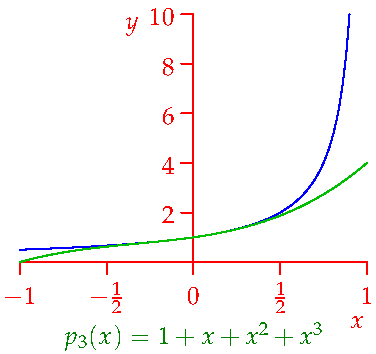
\includegraphics[scale=0.95]{taylor-remainder}
	\end{minipage}\medbreak
	If $x$ is close to 0, this is likely very small; for instance if $x\in\left[-\frac 12,\frac 12\right]$, then
	\[
		\nm{R_n(x)} \le\frac 1{1-\frac 12}\left(\frac 12\right)^{n+1} =2^{-n}
	\]
	However, when $x$ is close to 1 the error is unbounded!
\end{example}

The above behavior occurs in general: the truncated polynomials provide better approximations nearer the center of the series. To see this, we first need to consider higher-order derivatives.

\begin{defn}{}{}
	We write $f''$ for the \emph{second derivative} of $f$, namely the derivative of its derivative
	\[
		f''(a)=\lim_{x\to a}\frac{f'(x)-f'(a)}{x-a}
	\]
	The existence of $f''(a)$ presupposes that $f'$ exists on an (open) interval containing $a$. We can similarly consider third, fourth, and higher-order derivatives. As a function, the $n\th$ derivative is written
	\[
		f^{(n)}(x)=\diff[^nf]{x^n}
	\]
	By convention, the \emph{zeroth derivative} is the function itself $f^{(0)}(x)=f(x)$. We say that $f$ is \emph{$n$ times differentiable} at $a$ if $f^{(n)}(a)$ exists, and \emph{infinitely differentiable} (or \emph{smooth}) if derivatives of all orders exist.
\end{defn}

\begin{example}{}{}
	$f(x)=x^2\nm x$ is twice differentiable, with $f''(x)=6\nm x$. It is smooth everywhere except at $x=0$, where third (and higher-order) derivatives do not exist.
\end{example}


\goodbreak


\begin{defn}{}{}
	Suppose $f$ is $n$ times differentiable at $x=c$. The \emph{$n\th$ Taylor polynomial} $p_n$ of $f$ centered at $c$ is
	\[
		p_n(x):=\sum_{k=0}^n\frac{f^{(k)}(c)}{k!}(x-c)^k 
		=f(c)+f'(c)(x-c)+\frac{f''(c)}2(x-c)^2+\cdots+\frac{f^{(n)}(c)}{n!}(x-c)^n
	\]
	The \emph{remainder} $R_n(x)$ is the error in the polynomial approximation
	\[
		R_n(x)=f(x)-p_n(x)
		=f(x)-\sum_{j=0}^{n}\frac{f^{(k)}(c)}{k!}(x-c)^k
	\]
	If $f$ is infinitely differentiable at $x=c$, then its \emph{Taylor series} centered at $x=c$ is the power series
	\[
		\rT f(x) =\sum_{n=0}^\infty\frac{f^{(n)}(c)}{n!}(x-c)^n
	\]
	When $c=0$ this is known as a \emph{Maclaurin series.}\footnotemark
\end{defn}

\footnotetext{%
	Named for Englishman Brook Taylor (1685--1731) and Scotsman Colin Maclaurin (1698--1746). Taylor's general method expanded on examples discovered by James Gregory and Issac Newton in the mid-to-late 1600s.%
}

For simplicity we'll mostly work with Maclaurin series, with general situation hopefully being clear.

\begin{examples}{}{basictaylor}
	\exstart If $f(x)=e^{3x}$, then $f^{(n)}(x)=3^ne^x$, from which the Maclaurin series is
	\[
	  \rT f(x)=\sum_{n=0}^\infty\frac{3^n}{n!}x^n
	\]
	\begin{enumerate}\setcounter{enumi}{1}
	  \item If $g(x)=\sin 7x$, then the sequence of derivatives is
	  \[
	  	7\cos 7x,\ \ -7^2\sin 7x,\ \ -7^3\cos 7x,\ \ 7^4\sin 7x,\ \ 7^5\cos 7x,\ \ -7^6\sin 7x,\ \ldots
	  \]
		At $x=0$, every even derivative is zero whereas the odd derivatives alternate in sign. The Maclaurin series is easily seen to be
	  \[
	  	\rT g(x)=\sum_{n=0}^\infty\frac{(-1)^n7^{2n+1}}{(2n+1)!}x^{2n+1}
	  \]
	  
	  \item\label{ex:basictaylor3} If $h(x)=\sqrt x$, then $h'(x)=\frac 12x^{-1/2}$, $h''(x)=\frac{-1}{2^2}x^{-3/2}$, and $h'''(x)=\frac{3}{2^3}x^{-5/2}$, from which the third Taylor polynomial centered at $c=1$ is
	  \begin{align*}
	  	p_2(x)&=h(1)+h'(1)(x-1)+\frac{h''(1)}{2}(x-1)^2+\frac{h'''(1)}{6}(x-1)^3\\
	  	&=1+\frac 12(x-1)-\frac 18(x-1)^2+\frac 1{16}(x-1)^3
	  \end{align*}
	\end{enumerate}
\end{examples}

Rather than computing further examples, we first develop a little theory that makes verifying Taylor series much easier.
\goodbreak


	
\boldsubsubsection{Differentiation of Taylor Polynomials and Series}
	
Suppose $P(x)=\sum a_jx^j$ is a power series with radius of convergence $R>0$. As we saw previously (Theorem \ref{thm:psintdiff}), $P(x)$ is differentiable term-by-term on $(-R,R)$. Indeed,
\begin{gather*}
	%P(0)=a_0\\
	P'(x)=\sum_{j=1}^\infty a_jjx^{j-1} \implies P'(0)=a_1\\
	P''(x)=\sum_{j=2}^\infty a_jj(j-1)x^{j-2} \implies P''(0)=2a_2\\
	P'''(x)=\sum_{j=3}^\infty a_jj(j-1)(j-2)x^{j-3} \implies P'''(0)=3!a_3\\[-8pt]
	\quad\vdots\\[-3pt]
	P^{(k)}(x)=\sum_{j=k}^\infty a_jj(j-1)\cdots(j-k+1)x^{j-k}=\sum_{j=k}^\infty\frac{j!a_j}{(j-k)!}x^{j-k} \implies P^{(k)}(0)=k!a_k
\end{gather*}
Otherwise said, $P$ is its own Maclaurin series! The same discussion holds for polynomials. Indeed if $P(x)=a_0+a_1x+\cdots+a_nx^n$ is a polynomial and $f$ a function, then
\[
	P^{(k)}(0)=f^{(k)}(0)\iff a_k=\frac{f^{(k)}(0)}{k!}
\]
If this holds for \emph{all} $k\le n$, then $P=p_n$ is the $n\th$ Taylor polynomial of $f$! With a little modification, we've proved the following:

\begin{thm}{}{taylorlem}
	\exstart If $f(x)=\smash[b]{\sum\limits_{n=0}^\infty} a_n(x-c)^n$ on a neighborhood of $c$, then $\smash[b]{\sum\limits_{n=0}^\infty} a_n(x-c)^n$ is the Taylor series of $f$.
	\begin{enumerate}\setcounter{enumi}{1}
		\item The $n\th$ Taylor polynomial of $f$ centered at $x=c$ is the unique polynomial $p_n$ of degree $\le n$ whose value and first $n$ derivatives agree with those of $f$ at $x=c$: that is
		\[
			\forall k\le n,\ \ \smash[t]{p_n^{(k)}(c)=f^{(k)}(c)}
		\]
	\end{enumerate}
\end{thm}

This answers our first motivating question: a function can equal at most one power series with a given center. The second question requires a careful study of the \emph{remainder}: we'll do this shortly.

\begin{examples}{Common Maclaurin Series}{taylorexs}
	These should be familiar from elementary calculus. Each function equals the given series form our previous discussions of power series: by the Theorem, each series is immediately the Maclaurin series of the given function.
	\[
		\def\arraystretch{2}
		\begin{array}{ll@{\qquad\qquad\qquad}ll}
			\displaystyle e^x=\sum_{n=0}^\infty\frac{x^n}{n!} & x\in\R
			&\displaystyle\frac 1{1-x}=\sum_{n=0}^\infty x^n & x\in(-1,1)\\
			\displaystyle\sin x=\sum_{n=0}^\infty\frac{(-1)^n}{(2n+1)!}x^{2n+1} & x\in\R
			&\displaystyle\ln(1+x)=\sum_{n=1}^\infty \frac{(-1)^{n+1}}nx^n & x\in (-1,1]\\
			\displaystyle\cos x=\sum_{n=0}^\infty\frac{(-1)^n}{(2n)!}x^{2n} & x\in\R
			&\displaystyle\tan^{-1}x=\sum_{n=0}^\infty \frac{(-1)^n}{2n+1}x^{2n+1} & x\in[-1,1]
		\end{array}
	\]
\end{examples}


\goodbreak


\begin{examples}{Modifying Maclaurin Series}{modmaclaurin}
	By substituting for $x$ in a common series, we quickly obtain new series.
	\begin{enumerate}
	  \item Substitute $x\mapsto 7x$ in the Maclaurin series for $\sin x$, to recover our earlier example
	 	\[
	 		\sin 7x=\sum_{n=0}^\infty\frac{(-1)^n7^{2n+1}}{(2n+1)!}x^{2n+1},\quad x\in \R
	 	\]
		Note how this requires almost no calculation: since the function equals a series, the Theorem says we have the Maclaurin series for $\sin 7x$!
		
		\item Substitute $x\mapsto x^2$ in the Maclaurin series for $e^x$ to obtain
	  \[
	  	e^{x^2}=\exp(x^2)=\sum_{n=0}^\infty \frac{1}{n!}x^{2n},\quad x\in\R
	  \]
	  This would be disgusting to verify directly, given the difficulty of repeatedly differentiating $e^{x^2}$.
	  
	  \item We find the Taylor series for $f(x)=\frac 1{5-x}$ centered at $x=2$:
	  \[
	  	f(x)=\frac 1{3+2-x} =\frac 1{3(1-\frac{2-x}3)} =\frac 13\sum_{n=0}^\infty\left(\frac{2-x}3\right)^n
	  \]
	  which is valid whenever $-1<\frac{2-x}3<1\iff -1<x<5$.
	  
	  \item Fix $c\in\R$ and observe that, for all $x\in\R$,
	  \[
	  	e^x=e^{c+x-c}=e^ce^{x-c}=\sum_{n=0}^\infty \frac{e^c}{n!}(x-c)^n
	  \]
	  We conclude that the series is the Taylor series of $e^x$ centered at $x=c$. Of course this is easily verified using the definition, since $\diffat[^n]{x^n}{x=c}e^x=e^c$.
	  
	  \item Combining the Theorem with the multiple-angle formula, we obtain the Taylor series for $\sin x$ centered at $x=c$:
	  \begin{align*}
	  	\sin x&=\sin(c+x-c)
	  	=\sin c\cos(x-c)+\cos x\sin(x-c)\\
	  	&=\sum_{n=0}^\infty\frac{(-1)^n\sin c}{(2n)!}(x-c)^{2n} 
	  	+\sum_{n=0}^\infty\frac{(-1)^n\cos c}{(2n+1)!}(x-c)^{2n+1}
	  \end{align*}
	\end{enumerate}
\end{examples}


\begin{defn}{}{}
	A function $f$ is \emph{analytic} on a its domain if every $c\in\dom f$ has a neighborhood on which $f(x)$ equals its Taylor series centered at $c$.
\end{defn} 
	
All the examples we've thus far seen are analytic on their domains; indeed the last two of Examples \ref{ex:modmaclaurin} \emph{prove} this for the exponential and sine functions. Every analytic function is automatically smooth (infinitely differentiable), however the converse is \emph{false} (Exercise \ref{exs:macnoteq}). Analyticity is of greater importance in complex analysis where (amazingly!) it is equivalent to complex-differentiability.

\goodbreak


\boldsubsubsection{Accuracy of Taylor Approximations}

Our final goal is to estimate the accuracy of a Taylor polynomial as an approximation to its generating function. Otherwise said, we want to estimate the size of the remainder $R_n(x)=f(x)-p_n(x)$.

\begin{thm}{Taylor's Theorem: Lagrange's form}{taylor}
	Suppose $f$ is $n+1$ times differentiable on an open interval $I$ containing $c$ and let $x\in I\setminus\{c\}$. Then there exists $\xi$ between $c$ and $x$ for which the remainder centered at $c$ satisfies
	\[
		R_n(x)=\frac{f^{(n+1)}(\xi)}{(n+1)!}(x-c)^{n+1}
	\] 
\end{thm}

\begin{proof}
	For simplicity let $c=0$. Fix $x\neq 0$, define a constant $M_x$ and a function $g:I\to\R$ by
	\[
		R_n(x)=\frac{M_x}{(n+1)!}x^{n+1}
		\quad\text{and}\quad 
		g(t)=\frac{M_x}{(n+1)!}t^{n+1}+p_{n}(t)-f(t) 
		=\frac{M_x}{(n+1)!}t^{n+1}-R_{n}(t)
	\]
	Observe that
	\begin{align*}
		k\le n+1\implies 
		&g^{(k)}(x)=\frac{M_x}{(n+1-k)!}t^{n+1-k}+p^{(k)}_n(t)-f^{(k)}(t)\tag{$\ast$}\\
		\implies &g^{(k)}(0)=p^{(k)}_n(0)-f^{(k)}(0) =0
		\quad \text{if $k\le n$}
	\end{align*}
	where we invoked Theorem \ref{thm:taylorlem}.\smallbreak
	Now apply Rolle's Theorem repeatedly (WLOG assume $x>0$):
	\begin{itemize}
	  \item $\exists\xi_1$ between 0 and $x$ such that $g'(\xi_1)=0$.
	  \item $\exists\xi_2$ between 0 and $\xi_1$ such that $g''(\xi_2)=0$, etc.
	  \item Iterate to obtain a sequence $(\xi_k)$ such that
	  \[
	  	0<\xi_{n+1}<\xi_n<\cdots <\xi_1<x\quad\text{and}\quad g^{(k)}(\xi_k)=0
	  \]
	\end{itemize}
	Take $\xi=\xi_{n+1}$ and consider $(\ast)$: since $\operatorname{deg}p_n\le n$, we see that
	\[
		0=g^{(n+1)}(\xi)=M_x-f^{(n+1)}(\xi) 
		\implies R_n(x)=f(x)-p_n(x)
		=\frac{f^{(n+1)}(\xi)}{(n+1)!}x^{n+1}
		\tag*{\qedhere}
	\]
\end{proof}


\begin{cor}{}{}
	Suppose $f$ is smooth on an open interval $I$ containing $c$ and that all derivatives $f^{(n)}$ of all orders are bounded on $I$. Then $f$ equals its Taylor series (centered at $c$) on $I$.
\end{cor}

\begin{proof}
	For simplicity, let $c=0$. Suppose $\bigl|f^{(n+1)}(\xi)\bigr|\le K$ for all $\xi\in I$. Choose any $N>\nm{x}$ and observe that
	\[
		n>N \implies\nm{R_n(x)}\le\frac{K\nm{x}^{n+1}}{(n+1)!} 
		=\frac{K\nm x^{n+1}}{N!(N+1)\cdots(n+1)}
		\le\frac{K\nm x^{N}}{N!}\left(\frac{\nm x}{N}\right)^{n+1-N}
		\xrightarrow[n\to\infty]{} 0
		\tag*{\qedhere}
	\]
\end{proof}

%It is important to note that $\xi$ depends on $x$!


\goodbreak


\begin{examples}{}{}
	\exstart The functions sine and cosine have derivatives bounded by 1 on $\R$, and thus both functions equal their Maclaurin series on $\R$. This removes the need to have previously justified these facts using the theory of differential equations.
	\begin{enumerate}\setcounter{enumi}{1}
		\item The exponential function does not have bounded derivatives, however we can still apply Taylor's Theorem. For any fixed $x$, $\exists\xi$ between $0$ and $x$ such that
		\[
			\nm{R_n(x)}=\nm{\frac{e^\xi}{(n+1)!}x^{n+1}}
			\xrightarrow[n\to\infty]{} 0
		\]
		by the same argument in the Corollary. Thus $e^x$ equals its Maclaurin series on the real line (we knew this already from Exercise \ref{sec:derivproperties}.\ref{exs:expmasochist}).
		
		\item Extending Example \ref*{ex:basictaylor}.\ref*{ex:basictaylor3}, we see that $h(x)=\sqrt x$ has linear approximation (1\st{} Taylor polynomial) centered at $c=9$
		\[
			p_1(x)=h(9)+h'(9)(x-9)=3+\frac 16(x-9)
		\]
		This yields the simple approximation
		\[
			\sqrt{10}\approx p_1(10)= 3+\frac 16=\frac{19}6
		\]
		Taylor's Theorem can be used to estimate its accuracy (remember to shift the center to 9!):
		\[
			R_1(10)=\frac{h''(\xi)}{2!}(10-9)^2
			=-\frac{1}{2^2\cdot 2!}\xi^{-3/2} 
			=-\frac 1{8\xi^{3/2}}
			\quad\text{for some}\quad 
			\xi\in(9,10)
		\]
		Certainly $\xi^{-3/2}<9^{-3/2}=\frac 1{27}$, whence
		\[
			-\frac 1{216}<R_1(10)<0
			\implies \frac{19}6-\frac 1{216}
			=\frac{683}{216}<\sqrt{10}<\frac{684}{216}
			=\frac{19}6
		\]
		$\frac{19}6$ is therefore an overestimate for $\sqrt{10}$, but is accurate to within $\frac 1{216}<0.005$.
	\end{enumerate}
\end{examples}

%\vfil


\boldsubsubsection{Alternative Versions of Taylor's Theorem}

There are two further common expressions for the remainder in Taylor's Theorem. These are typically less easy to use than Lagrange's form but can sometimes provide sharper estimates for the remainder, particularly when $x$ is far from the center of the series.

\begin{cor}{}{}
	Suppose $f^{(n+1)}$ is continuous on an open interval $I$ containing $c$, let $x\in I\setminus\{c\}$, and let $R_n(x)=f(x)-p_n(x)$ be the remainder for the Taylor polynomial centered at $c$. Then:
	\begin{enumerate}
	  \item (Integral Remainder)\quad $\smash[b]{\displaystyle R_n(x)=\int_c^x\frac{(x-t)^n}{n!}f^{(n+1)}(t)\,\dt}$
		\item (Cauchy's Form)\quad $\exists\xi$ between $c$ and $x$ such that \
		$\displaystyle R_n(x)=\frac{(x-\xi)^{n}}{n!}(x-c)f^{(n+1)}(\xi)$
	\end{enumerate} 
\end{cor}

\goodbreak

Using these expressions it is possible to explicitly prove Newton's binomial series formula.

\begin{cor}{}{binomseries}
	If $\alpha\in\R$ and $\nm x<1$, then
	\begin{align*}
		(1+x)^\alpha
		&=1+\sum_{n=1}^\infty\frac{\alpha(\alpha-1)\cdots(\alpha-n+1)}{n!}x^n\\
		&=1+\alpha x+\frac{\alpha(\alpha-1)}{2!}x^2 
		+\frac{\alpha(\alpha-1)(\alpha-2)}{3!}x^3 
		+\frac{\alpha(\alpha-1)(\alpha-2)(\alpha-3)}{4!}x^4 +\cdots
	\end{align*}
\end{cor}

If $\alpha\in\N_0$, this is the usual binomial theorem. Otherwise it is more interesting: for instance,
\begin{gather*}
	\sqrt{1+x}=(1+x)^{1/2}=1+\frac 12x-\frac 18x^2+\frac 1{16}x^3-\frac 5{128}x^4+\cdots\\
	\frac 1{(1+x)^3}=1-3x+6x^2-10x^3+15x^4-\cdots
\end{gather*}
Of course this last could easily be obtained from $\frac 1{1+x}=\sum (-1)^nx^n$ by differentiating twice!

% \begin{proof}
% If $\alpha\in\N_0$, then the above is just a polynomial. Hence assume otherwise. First check that if $f(x)=(1+x)^\alpha$, then
% \[f^{(n)}(x)=\alpha(\alpha-1)\cdots(\alpha-n+1)(1+x)^{\alpha-n}\]
% from which it is clear that the above is the Maclaurin series of $f$. Now compute the radius of convergence,
% \[R=\lim_{n\to\infty}\nm{\frac{a_n}{a_{n+1}}}=\lim_{n\to\infty}\nm{\frac{n+1}{\alpha-n}}=1\]
% It follows that $a_nx^n\to 0$ for any $x\in(-1,1)$. Now consider Taylor's Theorem: for any $x\in(-1,1)$, $\exists\xi$ between $0$ and  $x$ for which
% \[\nm{R_n(x)}=\nm{\frac{f^{(n)}(\xi)}{n!}x^n}\]
% \end{proof}



\begin{exercises}
	\exstart Compute the Maclaurin series for $\cos x$ directly from the definition and use Taylor's Theorem to indicate why it converges to $\cos x$ for all $x\in \R$.
	\begin{enumerate}\setcounter{enumi}{1}
	  \item Repeat the previous exercise for $\sinh x=\frac 12(e^x-e^{-x})$ and $\cosh x=\frac 12(e^x+e^{-x})$.
	  
	  
	  \item Find the Maclaurin series for the function $\sin(3x^2)$. How do you know you are correct?
	  
	  
	  \item Find the Taylor series of $f(x)=x^4-3x^2+2x-5$ centered at $x=2$ and show that $\rT f(x)=f(x)$.
	  
	  
	  \item Find a rational approximation to $\sqrt[3]{9}$ using the first Taylor polynomial for $f(x)=\sqrt[3]{x}$. Now use Taylor's Theorem to estimate its accuracy.
	  
	  
	  \item If $c\neq 1$, use the fact that $1-x=(1-c)\left(1-\frac{x-c}{1-c}\right)$ to obtain the Taylor series of $\frac 1{1-x}$ centered at $c$. Hence conclude that $\frac 1{1-x}$ is analytic on its domain $\R\setminus\{1\}$.
	  
	  
	 	\item We use Taylor's Theorem to prove that the Maclaurin series $\smash[b]{\sum\limits_{n=1}^\infty} \frac{(-1)^{n+1}}nx^n$ converges to $\ln(1+x)$ whenever $0<x\le 1$.
	 	\begin{enumerate}
	 	  \item Explicitly compute $\diff[^{n+1}]{x^{n+1}}\ln(1+x)$. 
	 	  \item Suppose $0<x\le 1$. Using Taylor's Theorem, prove that $\lim\limits_{n\to\infty}R_n(x)=0$.
		\end{enumerate}
		(\emph{If $-1<x<0$, the argument is tougher, being similar to Exercise \ref{exs:binomialseries}})
		
		
		\item Why can't we use Taylor's Theorem to approximate the error in $\frac 1{1-x}=1+x+R_1(x)$ when $x\ge 1$? Try it when $x=2$, what happens? What about when $x=-2$?
	 	
	 	
		\item Prove Taylor's Theorem with integral remainder when $c=0$ by using the following as an induction step: for each $n\in\N$, define
	 	\[
	 		A_n(x)=\int_0^x\frac{(x-t)^n}{n!}f^{(n+1)}(t)\,\dt
	 	\]
	 	and use integration by parts to prove that $A_{n+1}=A_n-\frac{x^{n+1}}{(n+1)!}f^{(n+1)}(0)$.\par
	 	(\emph{The Cauchy form follows from the intermediate value theorem for integrals which we'll see later})
	 	
	 	
	 	\goodbreak
 	
 	
 		\item\label{exs:macnoteq} Consider the function
		\[
			f(x)=
			\begin{cases}
				e^{-1/x}&\text{if }x>0\\
				0&\text{otherwise}
			\end{cases}
		\]
		\begin{enumerate}
		  \item Prove by induction that there exists a degree $2n$ polynomial $q_n$ for which
			\[
				f^{(n)}(x)=q_n\left(\tfrac 1x\right)e^{-1/x}
				\text{ whenever }x>0
			\]
			\item Prove that $f$ is infinitely differentiable at $x=0$ with $f^{(n)}(0)=0$ (\emph{use Exercise \ref*{sec:lhopital}.\ref*{exs:pnexplimit}}).
		\end{enumerate}
		\emph{%
			The Maclaurin series of $f$ is identically zero! Moreover, $f$ is smooth (infinitely differentiable) on $\R$ but non-analytic at zero since it does not equal its Taylor series on any open interval containing zero.\\
			A modification allows us to create \emph{bump functions,} which find wide use in analysis. If $a<b$, define
			\[
				g_{a,b}:x\mapsto f(x-a)f(b-x)
			\]
		}

		\begin{minipage}[t]{0.6\linewidth}\vspace{-5pt}
			\emph{%
				This is smooth on $\R$ but non-zero only on the interval $(a,b)$. A further modification involving two such functions $g_{a,b}$ creates a smooth function on $\R$ which satisfies
				\[
					h_{a,b,\epsilon}(x)=
					\begin{cases}
						0&\text{if $x\le a-\epsilon$ or $x\ge b+\epsilon$}\\
						1&\text{if $a\le x\le b$}
					\end{cases}
				\]
				This `switches on' rapidly from 0 to 1 near $a$ and switches off similarly near $b$. By letting $\epsilon$ be small, we smoothly (but not uniformly) approximate the indicator function on $[a,b]$.%
			}
		\end{minipage}
		\hfill
		\begin{minipage}[t]{0.39\linewidth}\vspace{-20pt}
			\flushright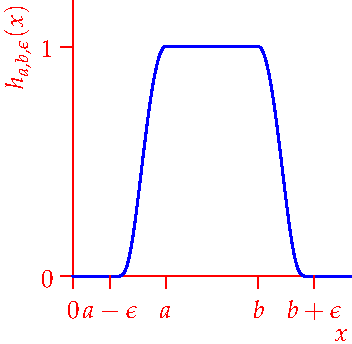
\includegraphics[scale=0.95]{diff-bump}
		\end{minipage}
	 	
	 	
	 	\item\label{exs:binomialseries} (Hard)\lstsp We prove the binomial series formula (Corollary \ref{cor:binomseries}).\par
	 	Let $f(x)=(1+x)^\alpha$ and $g(x)=1+\sum_{n=1}^\infty a_nx^n$ where $a_n=\frac{\alpha(\alpha-1)\cdots(\alpha-n+1)}{n!}$. Our goal is to prove that $f=g$ on the interval $(-1,1)$.
	 	\begin{enumerate}
	 	  \item Check that $f^{(n)}(0)=n!a_n$ so that $g$ really is the Maclaurin series of $f$.
	 	  
	 	  \item\begin{enumerate}
	 	    \item Prove that the radius of convergence of $g$ is 1.
	 	  	\item Prove that $\lim_{n\to\infty}na_nx^n=0$ whenever $\nm x<1$.
	 	  	\item If $\nm x<1$ and $\xi$ lies between 0 and $x$, prove that $\nm{\frac{x-\xi}{1+\xi}}\le\nm x$.\par
	 	  	(\emph{Hint: write $\xi=tx$ for some $t\in(0,1)$\ldots})
	 	  \end{enumerate}
	 	  
	 	  \item Use Taylor's Theorem with Cauchy remainder to prove that
	 	  \[
	 	  	\nm{R_n(x)}< (n+1)\nm{a_{n+1}}\nm x^{n+1}(1+\xi)^{\alpha-1}
	 	  \]
	 	  Hence conclude that $g=f$ whenever $\nm x<1$.
	 	  
	 	  \item Here is an alternative argument for the full result:
	 	  \begin{enumerate}
	 	    \item Show that $(n+1)a_{n+1}+na_n=\alpha a_n$.
	 	    \item Differentiate term-by-term to prove directly that $g$ satisfies the differential equation $(1+x)g'(x)=\alpha g(x)$. Solve this to show that $g=f$ whenever $\nm x<1$.
	 	  \end{enumerate}
	 	\end{enumerate}
	 	
	\end{enumerate}
\end{exercises}



 
% 
% One use of this example is in the creation of \emph{bump functions,} which find great use throughout analysis. If $f$ is the above function and $a<b$, then we may define the function
% \[g_{a,b}:x\mapsto f(x-a)f(b-x)\]
% 
% \begin{minipage}[t]{0.6\linewidth}\vspace{0pt}
% This function is infinitely differentiable on $\R$ but is non-zero only on the interval $(a,b)$. With a little modification, one can even create an infinitely differentiable function on $\R$ which satisfies
% \[h_{a,b,\epsilon}(x)=\begin{cases}
% 0&\text{if $x\le a-\epsilon$ or $x\ge b+\epsilon$}\\
% 1&\text{if $a\le x\le b$}
% \end{cases}\]
% This `switches on' from 0 to 1 over an interval of width $\epsilon$ near $a$, then switches off with similar rapidity near $b$. As $\epsilon\to 0$ this approximates the indicator function for the interval $[a,b]$.
% \end{minipage}\begin{minipage}[t]{0.4\linewidth}\vspace{0pt}
% \flushright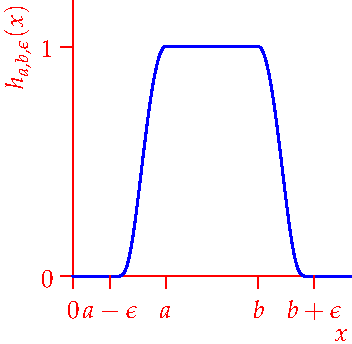
\includegraphics{diff-bump}
% \end{minipage}


% Indeed $g^{(n)}(\frac{a+b}2)=0$ for all $n\ge 1$, so one can even extend this: for any $a<b$ and $\epsilon>0$,
% \[h_{a,b,\epsilon}:x\mapsto \begin{cases}
% \frac 1{(g(a-\frac\epsilon 2))^2}g_{a-\epsilon,a}(x) & \text{if $x\in(a-\epsilon,a)$}\\
% 1&\text{if }a\le x\le b\\
% \frac 1{(g(b+\frac\epsilon 2))^2}g_{b,b+\epsilon}(x) & \text{if $x\in(b,b+\epsilon)$}\\
% 0 & \text{otherwise}
% \end{cases}\]
% 
% \begin{thm}[Taylor's theorem with integral remainder]
% Let $f$ be $n$ times differentiable on $(a,b)$ where $a<0<b$. Then for $x\in(a,b)$ we have
% \[R_n(x)=\int_0^x\frac{(x-t)^{n-1}}{(n-1)!}f^{(n)}(t)\D t.\tag*{$(\ast)$}\]
% \end{thm}
% 
% \begin{proof}
% We argue by induction. When $n=1$ we have $R_1(x)=f(x)-f(0)=\int_0^1f'(t)\D t$ (to be proved when we see the Fundamental Theorem of Calculus). Now assume that $(\ast)$ holds for some $n$. Then, by integration by parts (also to be justified later) we see that
% \begin{align*}
% R_n(x)&=\int_0^x\frac{(x-t)^{n-1}}{(n-1)!}f^{(n)}(t)\D t\\
% &=\left[-\frac{(x-t)^n}{n!}f^{(n)}(x)\right]_0^x+\int_0^x\frac{(x-t)^n}{n!}f^{(n+1)}(t)\D t\\
% &=\frac{x^n}{n!}f^{(n)}(x)+\int_0^x\frac{(x-t)^n}{n!}f^{(n+1)}(t)\D t.
% \end{align*}
% However this first term is precisely the difference $R_n(x)-R_{n+1}(x)$ from Definition \ref{defn:taylor}. Hence $(\ast)$ holds for $n+1$ and thus for all $n$ by induction.
% \end{proof}
% 
% Even though the result of the following example is easier to see directly from the previous corollary, we include it here for variety.
% 
% \begin{example}{}{}
% Let $f(x)=\sin x$. Then $\nm{f^{(n)}(x)}\le 1$ for all $x$. Hence
% \[\nm{R_n(x)}=\nm{\int_0^x\frac{(x-t)^{n-1}}{(n-1)!}f^{(n)}(t)\D t}\le\int_0^x\nm{\frac{(x-t)^{n-1}}{(n-1)!}}\D t=\frac{\nm x^n}{n!}\underset{n\to\infty}{\longrightarrow}0.\]
% Hence $\sin x$ is equal to its Taylor series for all $x\in\R$.



